\documentclass{book/custombook}
\unitname{Systems Programming}
\unitcode{CAB403}
\unitcoordinator{Timothy Chappell}
\author{Dinal Atapattu}
\begin{document}
    \maketitle
    \tableofcontents
    \chapter{Introduction to Operating Systems}
        \section{Operating System Structures}
            \subsection{Operating System Services}
                \begin{itemize}
                    \item Operating systems provide an environment for execution of programs and services to programs
                    and users
                    \item Operating System services provides functions that are helpful to the user
                        \begin{itemize}
                            \item User Interface - Almost all opeating systems have a user interface (UI)
                            \begin{itemize}
				\item Graphical (GUI)
                                \item Command Line (CLI)
                                \item Batch
                            \end{itemize}
                            \item Program Execution - The system must be able to load a program into memory and run that
                            program, end execution, either normally or abnormally (indicating error)
                            \item I/O operations - A running program may require I/O, which involves either a file or I/O device
                        \end{itemize}
                \end{itemize}
    \chapter{Operating System Structures}
	    An operating system provides the environment within which programs are executed. Internally, operating systems vary greatly in their makeup as they are organised to varying specifications.\\
        Operating systems are viewed from several points. Such as the services provided (users), the interface provided (programmers), and the components and their interconnections (operating system designers).\\
        \section{Operating System Services}
        \section{User and Operating System Interface}
            \subsection{Command Interpreters}
            \subsection{Touch Screen Interface}
        \section{System Calls}
            \subsection{Example}
            \subsection{API}
            \subsection{Types of syscalls}
    \chapter{Processes}
        Batch systems define a \textcolor{blue}{job} as a program and its data, and a time-shared system defines a \textcolor{blue}{task or user program}
        as the unit of work.\\
        Processes are programs in execution. The status of the current activity of a process is represented by the value of 
        the \textcolor{blue}{program counter} and the processor's registers. Programs are passive entities that are stored entirely in
        disk (\textcolor{blue}{executable fil}), programs become processses when the executable is loaded into memory.\\
        The memory layout of a process is divided into multiple sections, including
        \begin{itemize}
            \item \textbf{Text Section} - The program code
            \item \textbf{Data Section} - Global variables
            \item \textbf{Heap} - Dynamically allocated memory during runtime
            \item \textbf{Stack} - Temporary data such as function parameters, return addresses, and local variables
        \end{itemize}
        \begin{figure}[H]
            \centering
            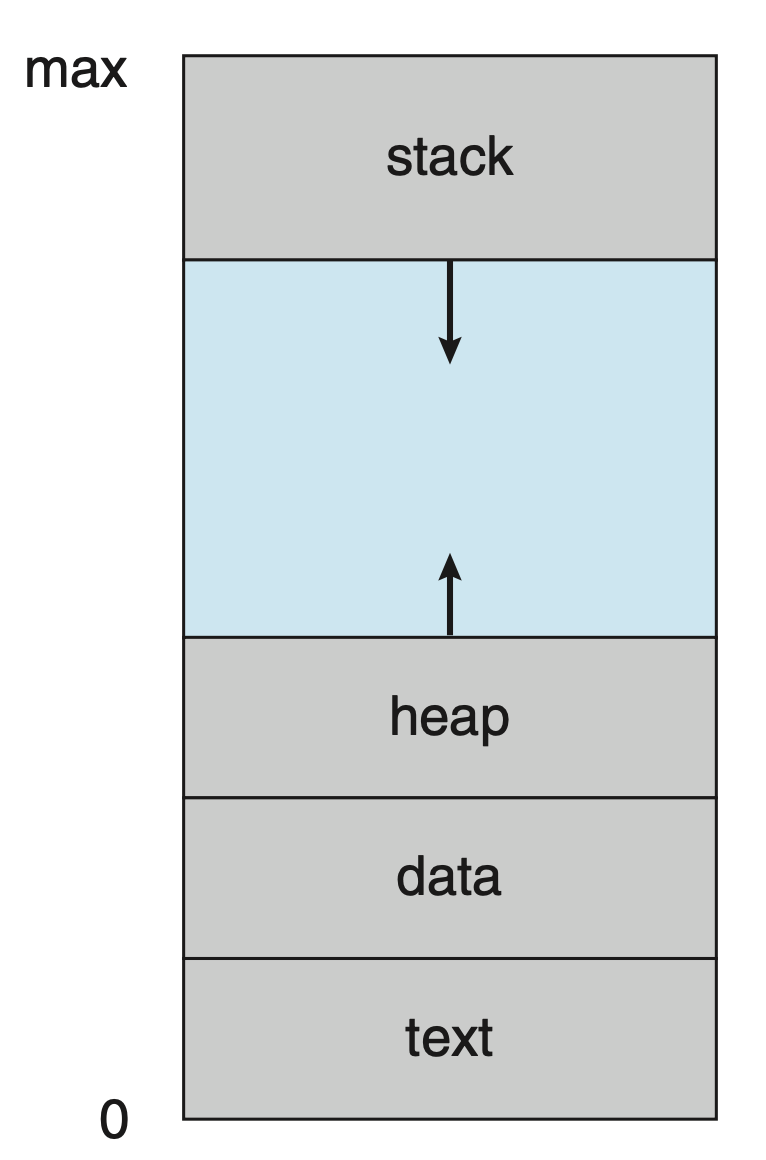
\includegraphics[width=0.2\linewidth]{figures/process_layout.png}
            \caption{Process Layout in Memory}
        \end{figure}
        The text and data sections are fixed size, while the heap and stack can change dynamically during runtime.
        Each time a function is called, an \textcolor{blue}{activation record} containing function parameters, local variables,
        and return address is pushed to the stack; when control is returned, the activation record is popped from the stack.
        While the heap and stack grow \textit{toward} each other, they are not allowed to collide (\textit{overlap}).\\
        \section{Process State}
            As a process executes, it changes \textcolor{blue}{state}. The state of a process is defined partly by the current 
            activity of the process. A process may be in one of the following states
            \begin{itemize}
                \item \textbf{New} - The process is being created
                \item \textbf{Running} - Instructions are being executed
                \item \textbf{Waiting} - The process is waiting for some event to occur (I/O completion, signal)
                \item \textbf{Ready} - The process is waiting to be assigned to a processor
                \item \textbf{Terminated} - The process has finished execution
            \end{itemize}
            \begin{figure}[H]
                \centering
                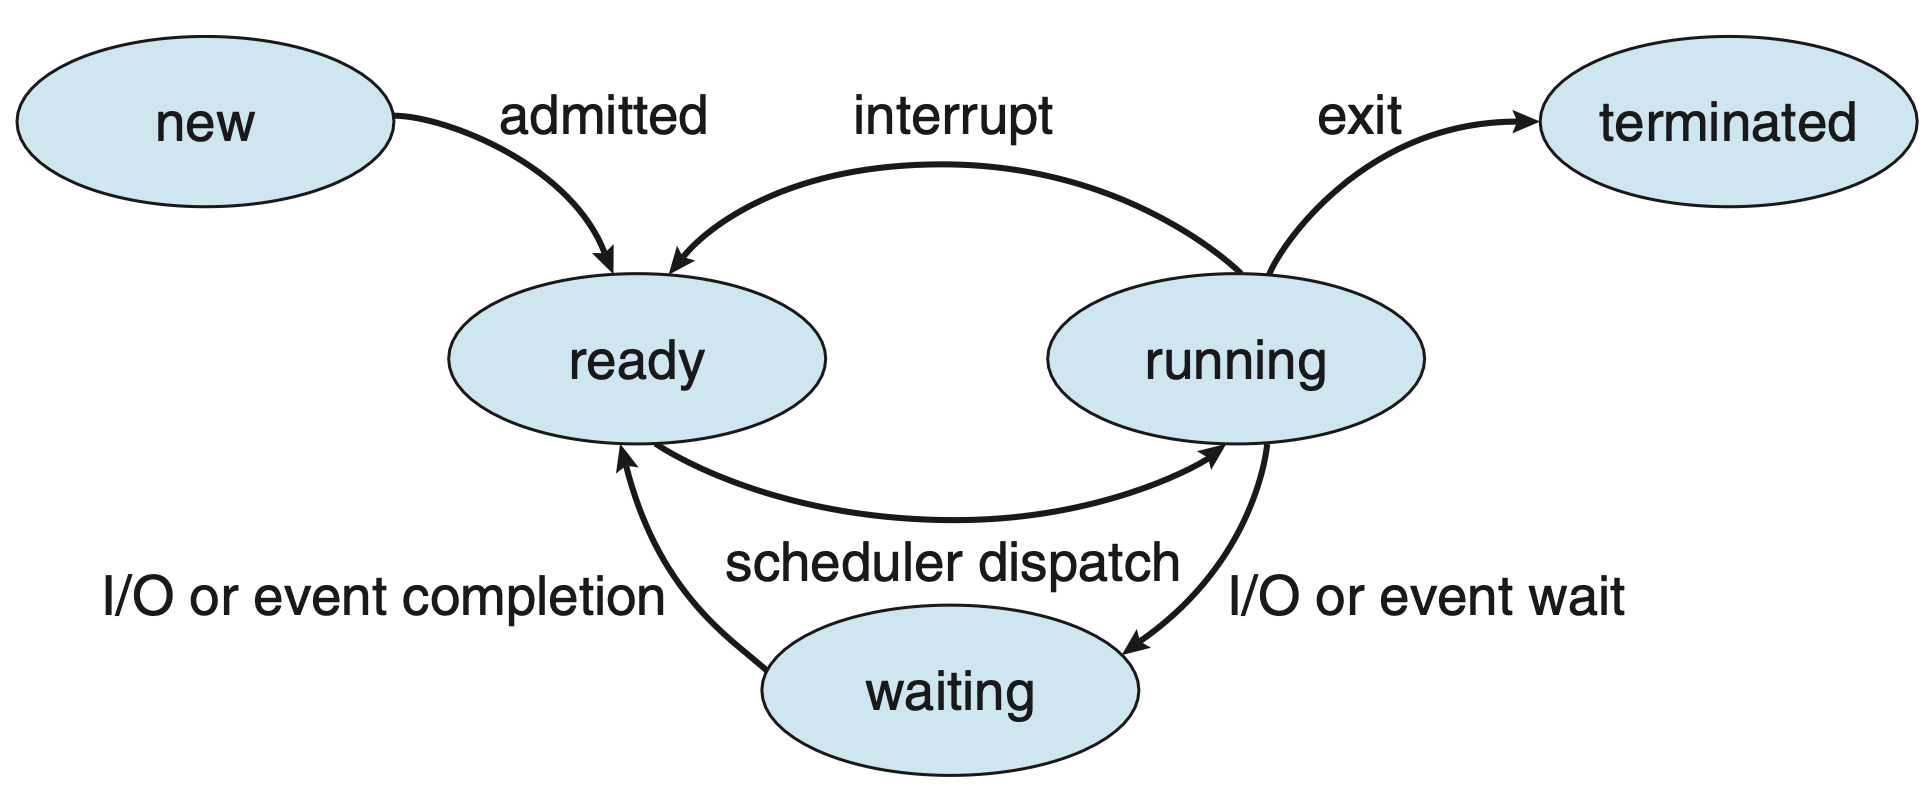
\includegraphics[width=0.6\linewidth]{figures/process_state.png}
                \caption{Process State Diagram}
            \end{figure}
            Only one process can be \textit{running} on any processor at any instant. Many processes may be \textit{ready} and \textit{waiting}.
        \section{Process Control Block}
            Each process is represented in the operting system by a \textcolor{blue}{process control block (PCB)} - also called a \textcolor{blue}{process control block},
            also called a \textcolor{blue}{task control block}.\\
            It contains many pieces of information associated with a specific process, including;
            \begin{itemize}
                \item \textbf{Process State} - New, Ready, Running, Waiting, Halted, Terminated, etc.
                \item \textbf{Program Counter} - Address of the next instruction to be executed for the process
                \item \textbf{CPU Registers} - Contents of all process-centric registers, these reisters vary from machine to machine and architecture to architecture. They include accumulators, index registers, stack pointers, and general-purpose registers, plus any condition code information. This state information must be saved along with the program counter when an interrupt occurs in order to allow the process to continue correctly after it is rescheduled to run
                \item \textbf{CPU Scheduling Information} - Process priority, pointers to scheduling queues, any other scheduling parameters
                \item \textbf{Memory Management Information} - Base and limit registers, page tables or segment tables, depending on the memory system used by the operating system. Depends on the memory system used by the operating system
                \item \textbf{Accounting Information} - Amount of CPU and real time used, time limits, account numbers, job or process numbers, etc.
                \item \textbf{I/O Status Information} - I/O Devices allocated to the process, list of open files, etc.
            \end{itemize}
            \begin{figure}[H]
                \centering
                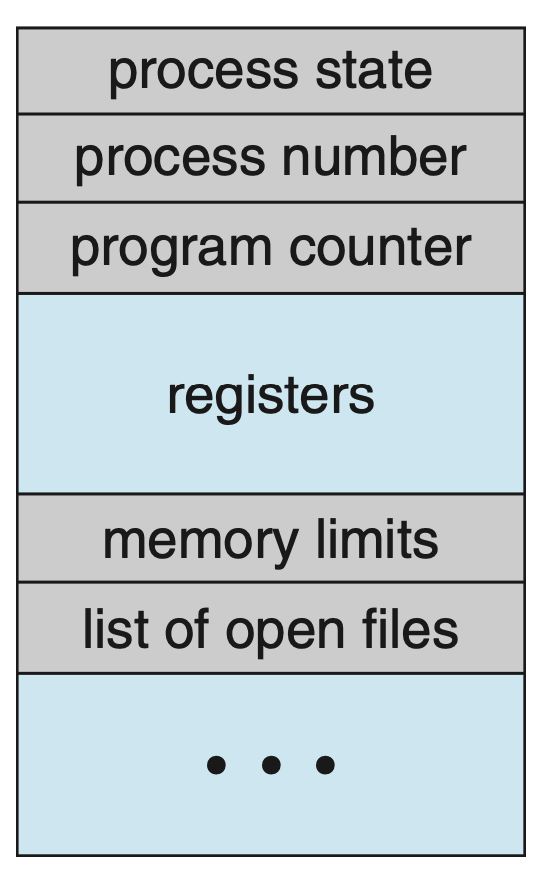
\includegraphics[width=0.2\linewidth]{figures/process_control_block.png}
                \caption{Process Control Block (PCB)}
            \end{figure}
        \section{Threads}
            In the process model, a process is a program that performs a single thread of exeuction. 
            A \textcolor{blue}{thread} is a basic unit of CPU utilization, consisting of a program counter,
            a stack, and a set of registers, and a thread ID. It shares with other threads belonging to the same
            process its code section, data section, and other operating-system resources, such as open files and signals.\\
            Modern operating systems have extended the process concept to allow a process on multiple threads of execution, allowing to perform more than one task at a time which is beneficial for multicore systems, where multiple threads can run in parallel. A multithreaded word process for example could, manage user input on one thread while another runs the spell checker.\\
            The PCB is expanded in these systems to include information for each thread, such as the thread ID, register set, and stack pointer, but the remaining information is shared among the threads within the same process.
        \section{Process Scheduling}
            The objective of multiprogramming is to have a process running at all times in order to maximize CPU utilization. The objective of time sharing is to switch the CPU among processes so frequently that users can interact with each program while it is running.\\
            These objectives are met using a \textcolor{blue}{process scheduler}, which selects an available process for program execution on a core. Each CPU core can run one process at a time.
    \chapter{Threads}
            A thread is a fundamental unit of CPU utilization, which forms the basis of multithreaded computer systems.
            Many modern applications are multithreaded, with threads running within an application. An application can divide tasks to seperate threads
            such as
            \begin{itemize}
                \item Updating the display
                \item Fetching data
                \item Spell checking
                \item Answering network requests
            \end{itemize}
            Thread creation, as opposed to process creation is lightweight, can simplify code, and increase efficiency. For this reason, kernels are often
            multithreaded.
            \begin{figure}[H]
                \centering
                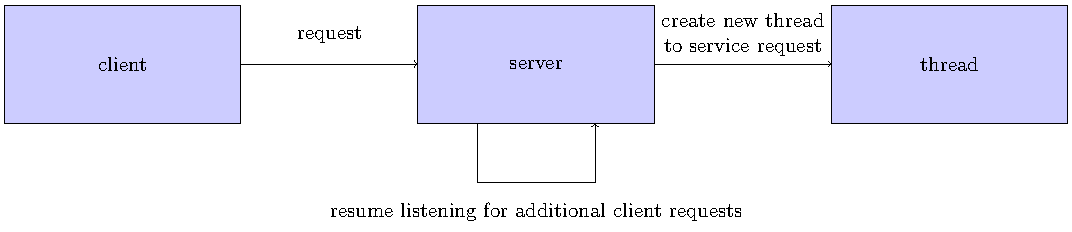
\includegraphics{figures/multithreader_server.pdf}
                \caption{Multithreaded Server Architecture}
            \end{figure}
            Multithreading has the following benefits
            \begin{itemize}
                \item \textbf{Responsiveness}
                    \subitem May allow continued execution if part of a process is blocked, important with user interfaces.
                \item \textbf{Resource Sharing}
                    \subitem Threads share resources of process, easier to manage than shared memory or message parsing.
                \item \textbf{Economy}
                    \subitem Cheaper than process creation, thread switching has lower overhead than context switching.
                \item \textbf{Scalability}
                    \subitem Processes can take advantage of a multiprocessor architecture
            \end{itemize}
        \section{Multicore Programming}
            In the early history of computer design, in order to combat the need for increased computing performance, single-CPU systems
            evoled into mult-CPU systems. Later, this evolved into including multiple compute cores on a single processing chip, where each core
            appears as a seperate CPU to the operating systems. These systems are defined as \textbf{multicore}.
            \subsection{Programming Challenges}
                The trend towards multicore systems continually places pressure on system designers and programmers to make better use of
                multiple compute cores. Designers of operating systems must write scheduling algorithms that use multiple processing cores
                to allow parallel execution
                \begin{figure}[H]
                    \centering
                    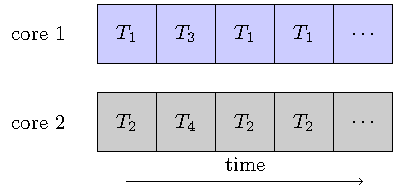
\includegraphics{figures/multicore_exec.pdf}
                    \caption{Parallel Execution on a Multicore System}
                \end{figure}
            In general, five areas present challenges in programming for multicore systems
            \begin{itemize}
                \item Identifying tasks
                    \subitem This involves examining applications to find areas that can be divided into seperate, concurrent tasks. Ideally, tasks
                    are independent of one another and thus can run in parallel on individual cores
                \item Balance
                    \subitem While Identifying tasks that run in parallel, programmers msut also ensure that tasks perform equal work of equal value.
                    In some instances, a certain task may not contribute as much value to the overall process as other tasks. Using seperate execution cores
                    for that task might not be worth the cost
                \item Data Splitting
                    \subitem Data accessed and manipulated by tasks must be divded to run on seperate cores, similar to how applications are divided to seperate tasks
                \item Data Dependency
                    \subitem The data accessed by he tasks must be examined for dependencies between the two or more tasks. When data is dependent between cores,
                    programmers must ensure that the execution of the tasks is synchronized to accomodate the dependency.
                    \begin{figure}[H]
                        \centering
                        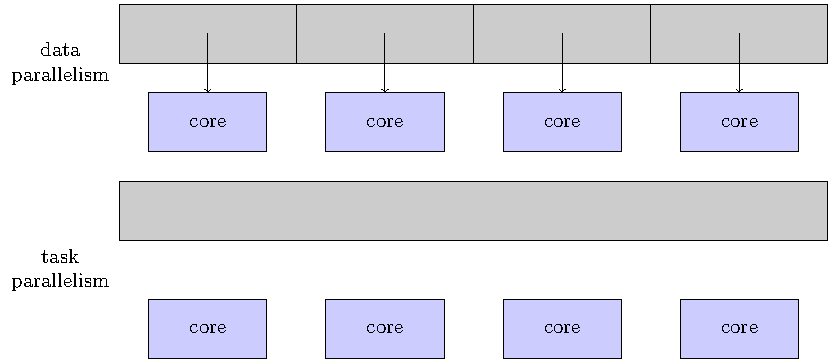
\includegraphics{figures/data_task_parallelism.pdf}
                        \caption{Data and Task Parallism}
                    \end{figure}
                \item Testing and Debugging
                    \subitem When a program is running in parallel n multiple cores, many different execution paths are possible. Testing and debugging such
                    concurrent programs is inherently more difficult than testing and debugging single threaded applications
            \end{itemize}
            \subsection{Parallelism}
                Types of parallelism
                \begin{itemize}
                    \item Data Parallelism
                        \subitem Focuses on distributing subsets of the same data across multiple compute cores, performing the same operation on each core.
                        \subitem Example: summing the contents of an array size $N$, on a dual core system, thread A sums the elements [0] ... [$N/2 - 1$], thread B
                        sums the elements $[N/2]$ ... $[N-1]$. These threads will run in parallel on seperate cores.
                    \item Task Parallelism
                        \subitem Distributes tasks across multiple cores. Each thread peforms a unique operation. Different threads may operate on the same or different
                        data.
                        \subitem Example: Dual core system, applying two different arithmetic and/or other operation on the same block of data on seperate threads. These
                        threads will will run parallel on seperate cores.
                \end{itemize}
                Data and Task parallelism may be done together, in a hybrid solution.
                \begin{figure}[H]
                    \centering
                    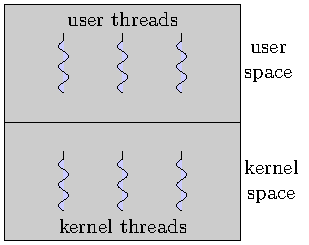
\includegraphics{figures/data_spaces.pdf}
                    \caption{Use and Kernel Data Spaces}
                \end{figure}
        \section{Multithreading Models}
            \subsection{Many-To-One Model}
                Many user-level threads are mapped to a single kernel thread.\\
                One thread block causes all to block.\\
                Multiple threads cannot run in parallel on a multicore system because the kernel can only handle a single thread.\\
                Rarely used.\\
                Examples include
                \begin{itemize}
                    \item Solaris Green threads
                    \item GNU Portable threads
                \end{itemize}
                \begin{figure}[H]
                    \centering
                    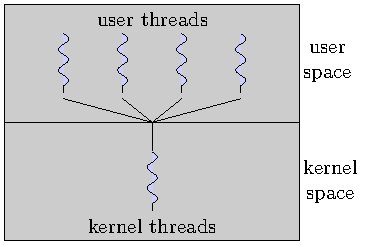
\includegraphics{figures/many_to_one.pdf}
                    \caption{Many-to-one model}
                \end{figure}
            \subsection{One-To-One Model}
                Each user-level thread maps to a kernel thread.\\
                Creating a user level thread creates a kernel thread.\\
                More concurrency than many-to-one.\\
                Number of threads per process sometimes restricted due to overhead.\\
                Examples include.
                \begin{itemize}
                    \item Windows
                    \item Linux
                    \item Solaris (9 and later)
                \end{itemize}
                \begin{figure}[H]
                    \centering
                    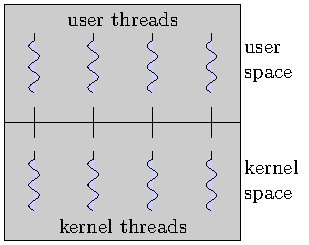
\includegraphics{figures/one_to_one.pdf}
                    \caption{One-to-one model} 
                \end{figure}
            \subsection{Many-to-many model}
                Allows many user level threads to be mapped to many kernel threads.\\
                Allows the operating system to create a sufficient number of kernel threads.\\
                Examples include
                \begin{itemize}
                    \item Solaris (pre version 9)
                    \item Windows (\textit{ThreadFiber} package)
                \end{itemize}
                \begin{figure}[H]
                    \centering
                    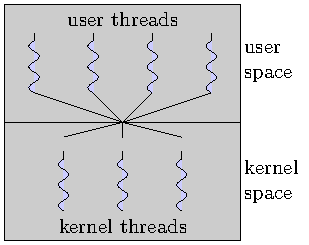
\includegraphics{figures/many_to_many.pdf}
                    \caption{Many-to-many model}
                \end{figure}
            \subsection{Two-level model}
                Similar to Many-to-many, except allows a user thread to be \textbf{bound} to a kernel thread
                Examples include
                \begin{itemize}
                    \item IRIX
                    \item HP-UX
                    \item Tru64 UNIX
                    \item Solaris (8 and earlier)
                \end{itemize}
                \begin{figure}[H]
                    \centering
                    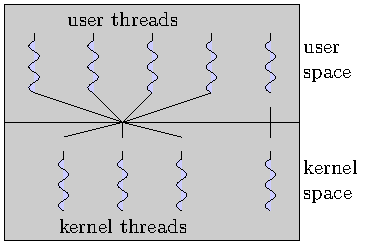
\includegraphics{figures/two_level.pdf}
                    \caption{Two-level model}
                \end{figure}
        \section{Thread Libraries}
            \subsection{Pthreads}
                Refers to the POSIX standard (IEEE 1003.1c) defining an API for thread creation and synchronisation.
                This is a specification not an implementation
                \begin{figure}[H]
                    \centering
                    \inputminted{c}{code/threads/pthreads.c}
                    \caption{Multithreading using the pthreads API}
                \end{figure}
                Although Windows does not natively support pthreads, some third-party implementations are available
                \begin{figure}[H]
                    \centering
                    \begin{minted}{c}
                        #define NUM_THREADS 10
                        /* an array of threads to be joined upon */
                        pthread_t workers[NUM_THREADS];

                        for (int i = 0; i < NUM_THREADS; i++)
                        {
                            pthread_join(workers[i], NULL);
                        }
                    \end{minted}
                    \caption{Joining 10 threads using the pthreads API}
                \end{figure}
            \subsection{Windows Threads}
                Similar to the technique used in pthreads. Uses a different library
                \begin{figure}[H]
                    \centering
                    \inputminted{c}{code/threads/windows_threads.c}
                    \caption{Multithreading using the Windows API}
                \end{figure}
        \section{Implicit Threading}
            The growing popularity of multicore processing means that applications now require hundreds,
            or thousands of threads. When designing such programs, correctness grows more and more difficult.
            Creating and management of threads done by compilers and run-time libraries are favoured in this case.
            \subsection{Thread Pools}
                Creates a number of threads in a pool where they await work
                Advantages
                \begin{itemize}
                    \item Usually faster to service a request with an existing thread than create a new thread
                    \item Alows the number of threads in an application(s) to be bound to the size of the pool
                    \item Seperating tasks to be performed from mechanics of creating task allows different stratgeies for
                    running task
                        \subitem Tasks could be scheduled to be run periodically
                \end{itemize}
                \begin{figure}[H]
                    \centering
                    \begin{minted}{c}
                        DWORD WINAPI PoolFunction(PVOID Param)
                        {
                            /*
                            * this function runs as a seperate thread
                            */
                        }
                    \end{minted}
                    \caption{Thread pooling in the Windows API}
                \end{figure}
            \subsection{OpenMP}
                Set of compiler directives and an API for C, C++, FORTRAN.\\
                Provides support for parallel programming and shared-memory environments.\\
                Identifies \textcolor{blue}{parallel regions} - blocks of code that can run in parallel.\\
                \begin{figure}[H]
                    \centering
                    \inputminted{c}{code/threads/openmp.c}
                    \caption{OpenMP}
                \end{figure}
            \subsection{Grand Central Dispatch}
                \begin{itemize}
                    \item Apple technology for Mac OS X and iOS operating systems
                    \item Extensions to C, C++, API and run-time library
                    \item Allows identification of parallel sections
                    \item Manages most details of threading
                    \item Blocks is in "\textasciicircum\{\}" - \mintinline{c}{^{ printf("I am a block"); }}
                    \item Blocks are placed in dispatch queue and then assigned to avaiable threads in thread pool when removed
                    \item Two types of dispatch queues
                        \begin{itemize}
                            \item \textbf{Serial} - blocks are removed FIFO, queue is per process, called \textbf{Main Queue}
                                \subitem Programmers create additional serial queues within program
                            \item \textbf{Concurrent} - removed in FIFO, but many be removed at a time
                                \subitem Three system wide queues with priorities \textcolor{blue}{low, default, high}
                                \begin{figure}[H]
                                    \begin{flushleft}
                                        \begin{minted}{c}
dispatch_queue_t queue = dispatch_get_global_queue(DISPATCH_QUEUE_PRIORITY_DEFAULT, 0);
dispatch_async(queue, ^{ printf("I am a block."); });
                                        \end{minted}
                                    \end{flushleft}
                                \end{figure}
                        \end{itemize}
                \end{itemize}
        \section{Threading Issues}
            \begin{itemize}
                \item Semantics of \textbf{fork()} and \textbf{exec()} system calls.
                \item Signal handling (synchronous and asynchronous)
                \item Thread cancellation of target thread (asynchronous or deferred)
                \item Thread local storage
                \item Scheduler activations
            \end{itemize}
            \subsection{Semantics of fork() and exec()}
                \begin{itemize}
                    \item Does fork() duplicate only the calling thread or all threads?
                        \subitem Some UNIXes have two versions of fork
                    \item exec() usually works as normal (replaces running process including all threads)
                \end{itemize}
            \subsection{Signal Handling}
                \begin{itemize}
                    \item \textcolor{blue}{Signals} are used in UNIX systems to notify a process that a particular event has occurred
                    \item A \textcolor{blue}{signal handler} is used to process signals
                        \begin{itemize}
                            \item Signal is generated by an event
                            \item Signal is delivered to a process
                            \item Signal is handled by one of two signal handlers
                                \subitem default
                                \subitem user-defined
                        \end{itemize}
                    \item Every signal has a \textcolor{blue}{default handler} that kernel runs when handling a signal
                        \begin{itemize}
                            \item \textcolor{blue}{User-defined signal handler} can override default
                            \item For single-threaded, signal delivered to process
                        \end{itemize}
                    \item Where is the signal delivered in multi-threaded?
                        \begin{itemize}
                            \item Deliver the signal to the thread to which the signal applies
                            \item Deliver the signal to every thread in the process
                            \item Deliver the signal to certain threads in process
                        \end{itemize}
                \end{itemize}
            \subsection{Thread Cancellation}
                \begin{itemize}
                    \item Terminating a thread before it has finished
                    \item Thread to be canceled is \textcolor{blue}{target thread}
                    \item Two general approaches
                        \begin{itemize}
                            \item \textbf{Asynchronous cancellation} terminates the target thread immediately
                            \item \textbf{Deferred cancellation} allows the target thread to periodically check if it should be cancelled
                        \end{itemize}
                        \begin{figure}[H]
                            \begin{minted}{c}
                                pthread_t thread_id;
                                /* create the thread */
                                pthread_create(&thread_id, 0, worker, NULL);
                                ...
                                /* cancel the thread */
                                pthread_cancel(thread_id);
                            \end{minted}
                            \caption{pthread code to create and cancel a thread}
                        \end{figure}
                    \item Invoking thread cancellation requests cancellation, but actual cancellation depends on the thread state
                        \begin{figure}[H]
                            \centering
                            \begin{tabular}{|c|c|c|}
                                \hline
                                \textbf{Mode} & \textbf{State} & \textbf{Type}\\
                                \hline
                                Off & Disabled & -\\
                                \hline
                                Deferred & Enabled & Deferred\\
                                \hline
                                Asynchronous & Enabled & Asynchronous\\
                                \hline
                            \end{tabular}
                            \caption{Thread States}
                        \end{figure}
                    \item If a thread has cancellation disabled, cancellation remains pending till enabled
                    \item Default type is deferred
                        \subitem Cancellation only occurs when thread reaches \textcolor{blue}{cancellation point}
                            \begin{itemize}
                                \item i.e., \mintinline{c}{pthread_testcancel();}
                                \item Then \textcolor{blue}{cleanup handler} is invoked
                            \end{itemize}
                    \item On Linux, thread cancellation is handled through signals
                \end{itemize}
            \subsection{Thread-Local Storage}
                \begin{itemize}
                    \item \textcolor{blue}{Thread-local-storage (TLS)} allows each thread to have its own copy of data
                    \item Useful when you don't have control over thread creation (i.e., using a thread pool)
                    \item Different from local variables
                        \begin{itemize}
                            \item Local variables visible only during single function invocation
                            \item TLS visible across function invocations
                        \end{itemize}
                    \item Similar to static data
                        \begin{itemize}
                            \item TLS is unique to each thread
                        \end{itemize}
                \end{itemize}
            \subsection{Scheduler Activations}
                \begin{itemize}
                    \item Both Many to Many and Two-Level require communication to maintain the appropriate 
                    number of kernel threads allocated to the application
                    \item Typically use an intermediate data structure between user and kernel threads (\textcolor{blue}{lightweight process (LWP)})
                        \begin{itemize}
                            \item Appears to be a virtual processor on which process can schedule user thread to run
                            \item Each LWP is attached to a kernel thread
                            \item How many LWPs to create?
                        \end{itemize}
                    \item Scheduler activations provide \textcolor{blue}{upcalls} - a communication mechanism from the kernel
                    to the \textcolor{blue}{upcall handler} in the thread library
                    \item This communication allows an application to maintain the correct number of kernel threads
                \end{itemize}
                \begin{figure}[H]
                    \centering
                    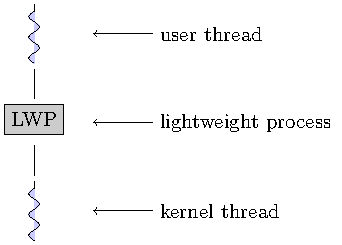
\includegraphics{figures/lwp.pdf}
                    \caption{Lightweight Process (LWP)}
                \end{figure}
    \chapter{Synchronisation}
        Processes can either execute concurrently or in parallel. These processes may be 
        interrupted at any time, partially completing execution.
        Concurrent access to any shared memory may result in data inconsistency if not properly
        controlled.\\
        Maintaining data consistency requires mechanisms to ensure the orderly execution of 
        cooperating processes.

        \hangindent=1cm Example: \\Suppose we wanted to provide a solution to the consumer-product problem that
        fills \textbf{all} the buffers. We can do so by having an integer \texttt{counter} that keeps
        track of the number of full buffers. Initially, \texttt{counter} is set to 0. It is incremented
        by the producer after producing a new buffer, and decremented by the consumer after it consumes
        a buffer.
        % side by side for producer consumer 2 figures each code blocks of C
        \begin{figure}[H]
            \centering
            \begin{subfigure}{0.5\textwidth}
                \begin{minted}[frame=lines, framesep=4mm, autogobble]{c}
                    while (true) {
                        /* produce an item in next produced */
                        while (counter == BUFFER_SIZE);
                            /* do nothing */
                        buffer[in] = next_produced;
                        in = (in + 1) % BUFFER_SIZE;
                        counter++;
                    }
                \end{minted}
            \end{subfigure}
            \begin{subfigure}{0.49\textwidth}
                \begin{minted}[frame=lines, framesep=4mm, autogobble]{c}
                    while (true) {
                        while (counter == 0);
                            /* do nothing */
                        next_consumed = buffer[out];
                        out = (out + 1) % BUFFER_SIZE;
                        counter--;
                        /* consume the item in next_consumed */
                    }
                \end{minted}
            \end{subfigure}
            \caption{Producer and Consumer}
        \end{figure}

        \section{Race Conditions}
        While the producer and consumer routines shown are correct seperately,
        they may not function correctly when executed concurrently.
        For example: Suppose that the value of the variable \texttt{count} is currently
        5 and the producer and consumer processes concurrently execute the statements
        "\texttt{count++}" and "\texttt{count--}". This will lead to the variable 
        being 4, 5 or 6. With the only correct value being \texttt{count == 5}, which 
        is executed if the producer and consumer execute seperately.
        We can show the value maybe incorrect by using the following implementation
            \begin{flalign*}
                register_1 &= count\\
                register_1 &= register_1 + 1\\
                count &= register_1\\
            \end{flalign*}
        where $register_1$ is one of the local CPU registers.\\
        Similarly, the statement \texttt{count - 1} is implemented as follows
            \begin{flalign*}
                register_2 &= count\\
                register_2 &= register_2 - 1;\\
                count &= register_2
            \end{flalign*}
        where again, $register_2$ is a local CPU register.\\
        \textcolor{red}{Even though $register_1$ and $register_2$ are local CPU registers, the value of
        this register will be saved and stored by the interrupt handler}\\
        The concurrent execution \texttt{count++} and \texttt{count -- 1} is equivalent
        to the sequential execution where lower evel statements previously are intef rleaved
        in an arbitrary order, with the order of the high-level statement is preserved.\
        \begin{figure}[H]
            \centering
            \begin{tabular}{c c c c c}
                $T_0$ & $producer$ & execute & $register_1 = count$ & \{$register_1$ = 5\}
            \end{tabular}
        \end{figure}
        \section{The Critical-Section Problem}
            In a system conssiting of \textit{n} processes \textit{$P_0, P_1, ... , P_{n-1}$}.
            Each process has a segment of code, called a \textcolor{blue}{critical section} in which
            the process is accessing and updating data that is shared with at least one process.
            The important feature of the system is that when one process is executing in its critical 
            section, no other process is allowed to execute in its critical section at the same time.\\
            The \textit{The critical section problem} is to design a protocol that processes can use to
            synchronize their activity to enter its critical section.\\
            It consists of the following sections
            \begin{itemize}
                \item \textcolor{blue}{Entry section} Implements requests for permission to enter its critical
                    section. Decides the entry of a particular process
                \item \textcolor{blue}{Critical Section} Part which only one process can enter and modify the
                    shared variable. This part of the process ensures that no other processes can access the 
                    shared resource
                \item \textcolor{blue}{Exit Section} Allows for other processes waiting in the entry section to
                    enter the critical section. It checks that a process if completed the critical section can move
                    to the remainder section
                \item \textcolor{blue}{Remainder Section} The other parts of the code, other than the entry, critical,
                    and exit sections
            \end{itemize}
            \subsection{Solution to the Critical Section Problem}
                A solution must satisfy the following 3 requirements
                \begin{itemize}
                    \item \textcolor{blue}{Mutual Exclusion}\\\\
                        \hspace*{1em}%
                            \begin{minipage}{0.8\textwidth}%
                                If process $\textit{P}_{\textit{i}}$ is executing in its critical section, then no other
                                process can be executing in their critical section
                            \end{minipage}%
                    \item \textcolor{blue}{Progress}\\\\
                        \hspace*{1em}%
                            \begin{minipage}{0.8\textwidth}%
                                If no process is executing in its critical section and some processes wish to 
                                enter their critical sections, then only those processes that are not executing in their
                                remainder sections can participate in deciding which will enter its critical section next,
                                and this selection cannot be postponed indefinitely.
                            \end{minipage}%
                    \item \textcolor{blue}{Bounded Waiting}\\\\
                        \hspace*{1em}%
                            \begin{minipage}{0.8\textwidth}%
                                There exists a bound, or limit, on the number of time that other processes are allowed to
                                enter their critical sections after a process has made a request to enter its critical
                                section and before that request is granted
                            \end{minipage}%
                \end{itemize}
           We assume that each process is executing at a nonzero speed. However, we can make no assumption about the
           relative speed of the processes.\\
           Many kernel-mode processes may be active in the operating system at the same time. As a result the kernel code
           (code implementing the operating system) may be subject to several possible race conditions.
    \chapter{Safety Critical Systems}
        \textbf{Safety} is the freedom from conditions that cause death, injury, illness, damage
        to or loss of equipment or property, or environmental harm\\
        Software is inherently not safe or unsafe, however can contribute to unsafe conditions in a
        safety critical system. Such software is \textbf{Safety Critical}\\
        IEEE definition: "Software whose use in a system can result in unacceptable risk. Safety-critical
        software incliudes softwre whose operation or failure to operate can lead to a hazardous state.
        Software intended to reover from hazardous states, and software intended to mitigate the severity
        of an incident"
        \section{MISRA C}
            \begin{itemize}
                \item Motor Industry Software Reliability Association
            \end{itemize}
        \section{NASA Power of 10}
            \begin{itemize}
                \item Avoid complex flow constructs (\textcolor{red}{goto, recursion, jumps})
                \item All loops must have fixed bounds (prevents runaway code)
                \item Avoid \textcolor{red}{heap memory allocation} (no malloc, define everything in main)
                \item Restrict functions to a single page (max 50 lines)
                \item Use a minimum of \textcolor{red}{two} runtime assertions per function
                \item Restrict the scope of data to the smallest possible
                \item Check the return value of all non-void functions, or cast to void to indicate the return is useless
                \item Use the preprocessor sparingly. (\textcolor{red}{DO NOT USE} stdio.h, local.h, abort/exit/system from stdlib.h, time handling from time.h)
                \item Limit pointer use to a \textcolor{red}{single dereference} and \textcolor{red}{DO NOT USE FUNCTION POINTERS}
                \item Compile with all warnings active (Wall, Wextra, etc.) all warnings should then be addressed before release
            \end{itemize}
    \chapter{Distributed Systems}
        A distributed system is a collection of processors that do not share memory or
        a clock. Instead, each node has its own local memory. The nodes communicate over 
        various networks, such as high-speed busses.\\
        Applications of distributed systems vary widely, from providing transparent file access
        inside an organization, to large-scale cloud storage services, to business analysis of 
        trends on large datasets, to parallel processing of scientific data. With the most 
        ubiqiutous form of a distributed system being the Internet.
        \section{Basic Concepts}
            A \textcolor{blue}{distributed system} is a collection of loosely coupled nodes
            interconnected by a communication network. From the point of view of a specific node
            in a distributed system, the rest of the nodes and their respective resources are remote,
            whereas its own resources are local.\\
            Processors are variously called \textbf{nodes, computers, machines, hosts}\\
            \begin{itemize}
                \item \textbf{Site} is the location of the processor
                \item Generally a \textbf{server} has a resource a \textbf{client} node at a different
                site wants to use
            \end{itemize}
            \begin{figure}[H]
                \centering
                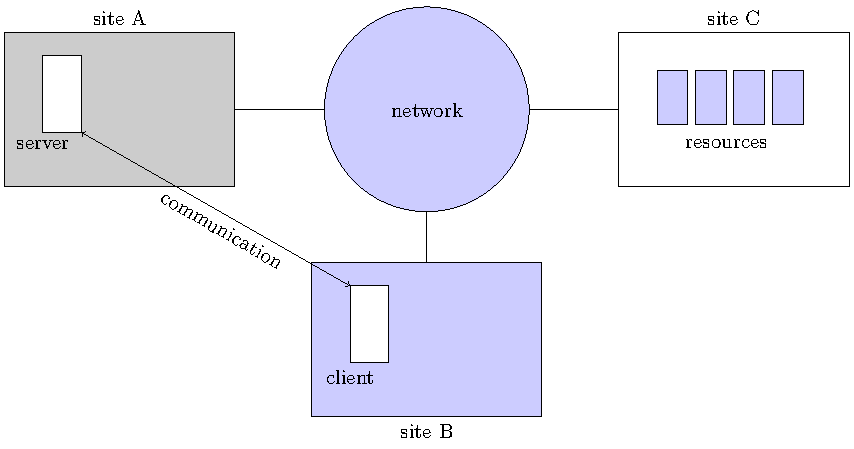
\includegraphics{figures/client_server.pdf}
                \caption{A client-server distributed system}
            \end{figure}
        \section{Advantages of Distributed Systems}
            \begin{itemize}
                \item \textbf{Resource Sharing}
                    \begin{itemize}
                        \item Sharing and printing files at remote sites
                        \item Processing information in a distributed database
                        \item Using remote specialized hardware devices
                    \end{itemize}
                \item \textbf{Computation speedup}
                    \begin{itemize}
                        \item \textbf{Load sharing}
                        \item \textbf{Job migration}
                    \end{itemize}
                \item \textbf{Reliability}
                    \subitem Detect and recover from site failure, function transfer,
                    reintegrate failed site.
                \item \textbf{Communication}
                    \subitem \textbf{Message passing}\\
                    \indent \indent All higher-level functions of a standalone system can
                    be expanded to encompass a distributed system
            \end{itemize}
            Computers can be downsized, more flexibility, better user interfaces and easier
            maintenance by moving from a large system to a cluster of smaller systems performing
            distributed computing
        \section{Network-Operating Systems}
        \section{Distributed Operating Systems}
    \chapter{CPU Scheduling}
        CPU scheduling is the basis of multiprogrammed operating systems.
        By switching the CPU among processes, the operating system can make the
        computer more productive.
        \section{Basic Concepts}
            A single core system can only run a single process at a time. Others must wait
            till the CPU's core is free and can be rescheduled.\\
            Multiprogramming is the idea of having a process running at all times to maximise
            CPU utilization.\\
            A process is executed until it must wait, typically for the completion of an I/O 
            request. A simple computer system just idles during this period, waiting compute time,
            no work is accomplished. With multiprogramming, we try to use this time productively.
            By keeping several processes in memory, when one process has to wait, the operating takes 
            the CPU away from the process and gives it to another process. On a multicore system this
            is extended to all processing cores on the system.\\
            Such scheduling is fundamental to an operating system's functionality. Almost all 
            computer resources are scheduled before use. The CPU, being one of the primary resources
            of a computer needs special attention during its scheduling
            \begin{figure}[H]
                \centering
                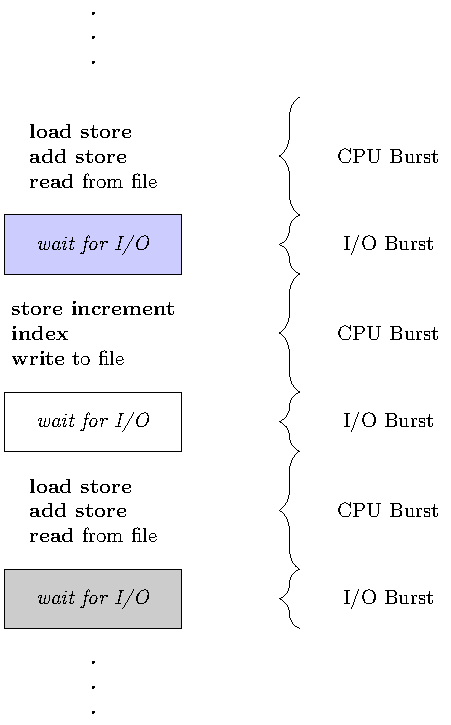
\includegraphics[width=0.2\linewidth]{figures/cpu_io_burst.pdf}
                \caption{Alternating Sequence of CPU and I/O Bursts}
            \end{figure}
            % \subsubsection{CPU-I/O Burst Cycle}
        \section{CPU Scheduler}
            Whenever the CPU idles, the operating system must select a process in the ready queue to be 
            executed.\\
            This is selected by the \textcolor{blue}{CPU Scheduler}. Which selects a process from the processes
            in memory that are ready to execute, and allocates the CPU to it.\\
            The \textcolor{blue}{short-term scheduler} seelcts from processes in the ready queue and allocates 
            the CPU to one of them.\\
            CPU scheduling happens when
            \begin{itemize}
                \item Switching from running to waiting
                \item Switching from running to ready
                \item Switching from waiting to ready
                \item Terminating
            \end{itemize}
            \subsection{Preemptive and Non-Preemptive Scheduling}
                CPU-scheduling decisions may take place under the following four circumstances
                \begin{enumerate}
                    \item Process switching from running state to the waiting state (I/O request, wait invocation for Terminating
                    a child process)
                    \item Process switching from running to ready state (interrupt)
                    \item Process switching from waiting to ready (I/O completion, release of a             \subsection{API}
                        \subsection{Types of syscalls}
        semaphore)
                    \item Process terminating
                \end{enumerate}
                For circumstances 1 and 4, there is no choice in scheduling, a new process (if exists) must be
                selected for execution. For circumstances 2 and 3, a choice exists.\\
                Circumstance 1, and 4 are called \textcolor{blue}{non preemptive} or \textcolor{blue}{cooperative}.
                Otherwise it is \textcolor{blue}{preemptive}.\\
                \textcolor{blue}{Non-preemptive} scheduling keeps the CPU once the process is allocated till termination
                or switching to the wait state.

                \subsubsection{Preemptive Scheduling}
                    Virtually all modern operating systems use preemptive scheduling.\\
                    However, Preemptive scheduling can result in \textcolor{red}{race conditions} when
                    data is shared between processes (first process is updating data while the second process
                    tries to read it, which is in an inconsistent state).\\
                    Kernel design must be modified to accomodate a preemptive scheduler as race conditions
                    in updating or modifying important kernel data (IO queues, process table, etc.) while they 
                    are being read can cause the system to crash.\\
                    Therefore, a preemptive kernel requires mechanisms such as mutex locks to prevent race conditions
                    when accessing shared kernel data structues.\\
                    Most modern operating systems are \textcolor{blue}{full prememptive} when running in kernel mode.
                \subsubsection{Non Preemptive Scheduling}
                    Non preemptive scheduling is simpler than preemptive scheduling as there is no need 
                    for any special hardware or kernel mode privileges.\\
                    However, non preemptive scheduling is not suitable for modern operating systems as it   
                    does not allow the kernel to respond to interrupts while running in kernel mode.\\
                    Non preemptive scheduling is used in embedded systems where the kernel is the only process
                    running on the system.\\
                    Non preemptive scheduling is also used in real time systems where the kernel is the only process 
                    running on the system.\\
        \section{Dispatcher}
            Is the module that gives control of the CPU's core to the process selected by the scheduler.
            Involves
            \begin{itemize}
                \item Context switching
                \item Switching to user model
                \item Jumping to the proper location in the user program to resume that program
            \end{itemize}
            Speed is crucial with the dispatcher as it is invoked during every context switch.\\
            \textcolor{blue}{Dispatch latency} is the time taken for the dispatcher to stop one process and
            starty another running.\\
        \section{Scheduling}
            Optimisation objectives
            \begin{itemize}
                \item Max CPU utilization
                \item Max throughput
                \item Min turnaround time
                \item Min waiting time
                \item Min response time
            \end{itemize}
            \subsection{First-Come, First-Served (FCFS) Scheduling}
                The process that requests the CPU first is allocated the CPU first.\\
                Managed using a FIFO queue.\\
                Given the following process table
                \begin{figure}[H]
                    \centering
                    \begin{subfigure}{0.5\textwidth}
                        \centering
                        \begin{tabular}{ccc}
                            Process & Burst Time & Arrival Time\\
                            \toprule
                            P1 & 24 & 0\\
                            P2 & 3  & 1\\
                            P3 & 3  & 2\\
                            \bottomrule
                        \end{tabular}
                        \caption{Process Table}
                    \end{subfigure}%
                    \begin{subfigure}{0.5\textwidth}
                        \centering
                        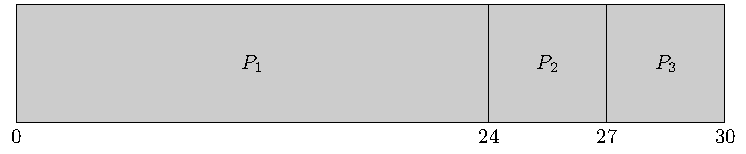
\includegraphics[width=\linewidth]{figures/fifo_gantt_1.pdf}
                        \caption{FIFO Gantt Chart}
                    \end{subfigure}
                    Waiting time for $P_1$ is 0, $P_2$ is 24, $P_3$ is 27. Average waiting time is 17.
                    \caption{Process Table and FIFO Gantt Chart with waiting times}
                \end{figure}
                \begin{figure}[H]
                    \centering
                    \begin{subfigure}{0.5\textwidth}
                        \centering
                        \begin{tabular}{ccc}
                            Process & Burst Time & Arrival Time\\
                            \toprule
                            P1 & 24 & 3\\
                            P2 & 3  & 1\\
                            P3 & 3  & 2\\
                            \bottomrule
                        \end{tabular}
                        \caption{Process Table}
                    \end{subfigure}%
                    \begin{subfigure}{0.5\textwidth}
                        \centering
                        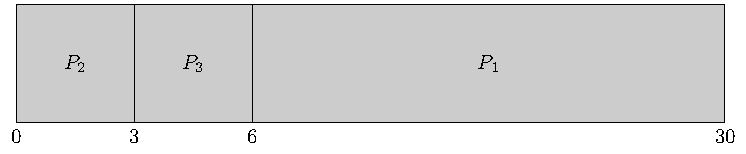
\includegraphics[width=\linewidth]{figures/fifo_gantt_2.pdf}
                        \caption{FIFO Gantt Chart}
                    \end{subfigure}
                    Waiting time for $P_1$ is 6, $P_2$ is 0, $P_3$ is 3. Average waiting time is 3.
                    \caption{Process Table and FIFO Gantt Chart with waiting times}
                \end{figure}
            \subsection{Shortest-Job-First (SJF) Scheduling}
                By associating each process with the length of its next CPU burst, we can schedule the process
                with the shortest time.\\
                SJF is optimal, giving the minimum average waiting time for a given set of processes.\\
                However, knowing the length of the next CPU burst is difficult to predict the length of the next
                CPU burst.\\
                \begin{figure}[H]
                    \centering
                    \begin{subfigure}{0.5\linewidth}
                        \centering
                        \begin{tabular}{cc}
                            Process & Burst Time\\
                            \toprule
                            P1 & 6\\
                            P2 & 8\\
                            P3 & 7\\
                            P4 & 3\\
                        \end{tabular}
                        \caption{Process Table}
                    \end{subfigure}%
                    \begin{subfigure}{0.5\linewidth}
                        \centering
                        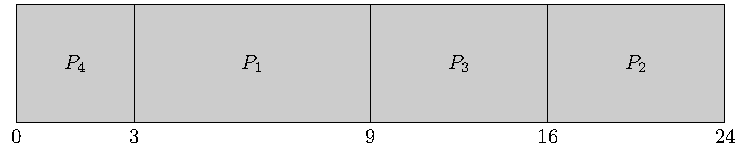
\includegraphics[width=\linewidth]{figures/sjf_gantt_1.pdf}
                        \caption{SJF Gantt Chart}
                    \end{subfigure}
                    Average waiting time is 7
                    \caption{Process Table and SJF Gantt Chart with waiting times}
                \end{figure}
                SJF can be either preemptive or non preemptive.\\
                Preemptive SJF is also called \textcolor{blue}{Shortest Remaining Time First}
                \begin{figure}[H]
                    \centering
                    \begin{subfigure}{0.5\linewidth}
                        \begin{tabular}{ccc}
                            Process & Arrival Time & Burst Time\\
                            \toprule
                            P1 & 0 & 8\\
                            P2 & 1 & 4\\
                            P3 & 2 & 9\\
                            P4 & 3 & 5\\
                        \end{tabular}
                        \caption{Process Table with Arrival Time}
                    \end{subfigure}%
                    \begin{subfigure}{0.5\linewidth}
                        \centering
                        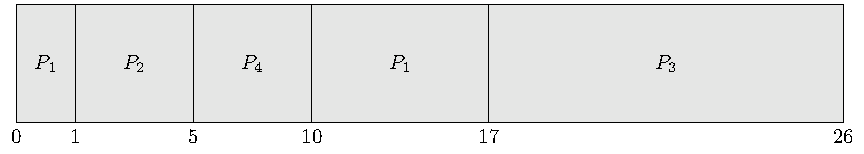
\includegraphics[width=\linewidth]{figures/srtf_gantt_1.pdf}
                        \caption{SRTF Gantt Chart}
                    \end{subfigure}
                    Average waiting time is 6.5
                    \caption{Process Table and SRTF Gantt Chart with waiting times}
                \end{figure}
            \subsection{Round Robin Scheduling}
                Each process is given a small unit of CPU time (\textcolor{blue}{time quantum} or \textcolor{blue}{time slice} q) that
                is 10-100 millisecond.
                After that time, the process is preempted and added to the end of the ready queue.\\
                If there are n processes in the ready queue and the time quantum is q, then each process
                gets 1/n of the CPU time in chunks of at most q time units at once. No process waits more
                than (n-1)q time units.\\
                Timer interrupts every quantum to schedule the next process.\\
                \begin{figure}[H]
                    \centering
                    \begin{subfigure}{0.5\linewidth}
                        \centering
                        \begin{tabular}{cc}
                            Process & Burst Time\\
                            \toprule
                            P1 & 24\\
                            P2 & 3\\
                            P3 & 3\\
                        \end{tabular}
                        \caption{Process Table}
                    \end{subfigure}%
                    \begin{subfigure}{0.5\linewidth}
                        \centering
                        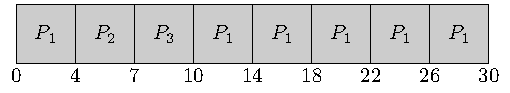
\includegraphics{figures/rr_time_quant_4.pdf}
                        \caption{Round Robin Gantt Chart}
                    \end{subfigure}
                    \caption{Round Robin Gantt Chart with time quantum 4}
                \end{figure}
                Typically, round robin has a higher average turnaround than SJF but has better reponse.
    \chapter{Deadlocks}
        \section{System Model}
            A system consists of finite resources distributed among a number of competing threads.
            These resources must be partitioned into several types or classes, each consisting of identical
            instances.\\
            Under normal operation, a thread may utilize a resource in the following sequence
            \begin{enumerate}
                \item \textbf{Request} - The thread requests the resource. If the request cannot be granted 
                immediately (for example, if a mutex lock is held by another thread) the requesting thread must
                wait till it can acquire the resource.
                \item \textbf{Use} - The thread can operate on the resource (for example, if the resource is a mutex
                lock, it can access its critical section)
                \item \textbf{Release} - The thread releases the resource (for example, if the resource is a mutex
                lock, it releases the lock, allowing another thread to acquire it)
            \end{enumerate}
        \section{Deadlock Characterization}
            Deadlocks can arise if four conditions hold simultaneously
            \begin{itemize}
                \item \textbf{Mutual exclusion} - At least one resource must be held in a nonsharable mode;
                that is, only one thread ata time can use the resource. If another thread requests that resource, 
                the requesting thread must be delayed until the resource is released.
                \item \textbf{Hold and Wait} - A thread must be holding at least one resource and waiting to acquire
                additional resources that are currently being hld by other threads
                \item \textbf{No Preemption} - Resources cannot be preempted; resources can only be released voluntarily
                by the thread holding it, after that the thread has completed its task.
                \item \textbf{Circular Wait} - A set of waiting threads must exist such that $T_0$ is waiting for a 
                resource held by $T_1$, $T_1$ is waiting for a resource held by $T_2$, ... $T_{n-1}$ is waiting for a 
                resource held by $T_n$, and $T_n$ is waiting for a resource held by $T_0$.
            \end{itemize}
            Note that circular wait implies hold and wait
        \section{Resource-Allocation Graph}
            A set of vertices V and a set of edges E.
            \begin{itemize}
                \item V is partitioned into two types
                    \subitem P - Set consisting of all the threads in the system
                    \subitem R - Set consisting of all resource types in the system
                \item \textbf{Request edge}
                    \subitem Directed edge $T_i \rightarrow R_j$
                \item \textbf{Assignment edge}
                    \subitem Directed edge $R_j \rightarrow T_i$
            \end{itemize}
            \begin{figure}[H]
                \centering
                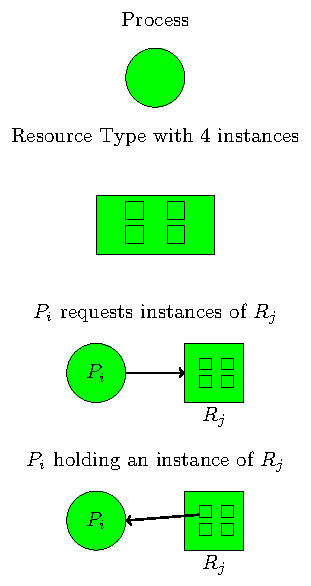
\includegraphics{figures/resource_allocation_graph.pdf}
                \caption{Resource Allocation Graph}
            \end{figure}
            \begin{figure}[H]
                \centering
                \begin{subfigure}{0.5\linewidth}
                        \centering
                        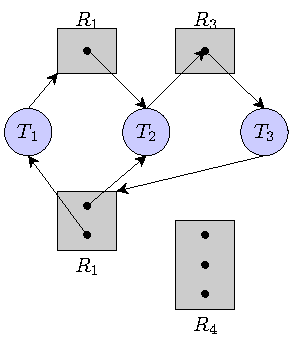
\includegraphics{figures/deadlock_resource_alloc_graph.pdf}
                        \caption{Resource Allocation Graph with Deadlock}
                \end{subfigure}%
                \begin{subfigure}{0.5\linewidth}
                        \centering
                        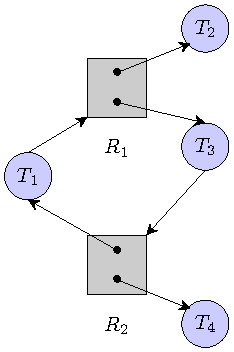
\includegraphics{figures/no_deadlock_resource_alloc_graph.pdf}
                        \caption{Resource Allocation Graph without Deadlock}
                \end{subfigure}
                \caption{Resource Allocation Graphs}
            \end{figure}
            \subsection{Basic Facts}
                \begin{itemize}
                    \item If a graph has no cycles there is no deadlock
                    \item If a graph has a cycle
                        \subitem If only one instance per resource type, then there's a deadlock
                        \subitem If several instances per resource type, then deadlock may or may not exist
                \end{itemize}
        \section{Methods for Handling Deadlocks}
            Ensure the system will never enter a deadlock state, or make sure that once a deadlock occurs,
            it will be recovered from the state. OR ignore the problem and pretend that deadlocks never occur
            in the system (UNIX, Linux, Windows).\\
        \section{Deadlock Prevention}
            Restrain the way requests can be made
            \begin{itemize}
                \item \textbf{Mutual Exclusion} - Not required for sharable resources, must hold for nonsharable
                resources
                \item \textbf{Hold and Wait} - Must guarantee that whenever a thread requests a resource, it does
                not hold any other resources
                    \begin{itemize}
                        \item Require that each thread request all its resources at one time
                        \item Require that once a thread holds a resource, it cannot request additional resources
                        \item Require that once a thread requests a resource, it cannot request additional resources
                        till the requested resource has been allocated to it
                    \end{itemize}
                \item \textbf{No preemption}
                    \begin{itemize}
                        \item If a process that is holding some resources requests another resource that cannot immediately
                        allocated to it, then all resources held must be released.
                        \item Preempted resources are added to the list of resources for which the process is waiting
                        \item Process will be restarted only when it can regain old resources, as as the ones requested
                    \end{itemize}
                \item \textbf{Circular Wait}
                    \begin{itemize}
                        \item Impose a total ordering of all resource types, and require that each thread requests resources
                        in an increasing order of enumeration
                    \end{itemize}
            \end{itemize}
        \section{Deadlock Avoidance}
            Requires that the system has some additional \textbf{a priori} information available.\\
            \begin{itemize}
                \item Simplest and most useful model requires that each process declare the \textbf{maximum number} of resources
                of each type it may need
                \item The deadlock-avoidance algorithm dynamically examines the resource-allocation state to ensure that there can
                never be a circular-wait condition
                \item Resource-allocation state is defined by the number of available and allocated resources, and the maximum demands
                of the processes/threads.
            \end{itemize}
            \subsection{Basic Facts}
                \begin{itemize}
                    \item If a system is in safe state, no deadlocks
                    \item If a system is in unsafe state, possibility of deadlock
                    \item Avoidance, ensure that a system will never enter an unsafe state
                \end{itemize}
        \section{Safe State}
            When a process requests and available resource, the system must decide if immediate allocation leaves the system in 
            a safe state.\\
            The system is in a \textbf{safe state} if there exists a sequence of \textbf{ALL} the processes in the system such that
            for each $P_i$, the resources that $P_i$ can still request can be satisfied by currently available resources + resources 
            held by all the $P_j$, with $j < i$. i.e.,
            \begin{itemize}
                \item If $P_i$ requests a resource, it may have to wait till all the $P_j$ with $j < i$ have finished
                \item When $P_j$ is finished, $P_i$ can obtain its needed resources, execute, return allocated resources, and terminate
                \item When $P_i$ terminates, $P_{i+1}$ can obtain its needed resources, and so on
            \end{itemize}
        \section{Deadlock Avoidance Algorithms}
            \subsection{Resource Allocation Graph Scheme}
                \begin{itemize}
                    \item \textcolor{blue}{Claim edge} $P_i \rightarrow R_j$ indicated that processes $P_i$ may request resource
                    $R_j$.
                    \item Claim edge converts to request edge when a process/thread requests a resource.
                    \item Request edge converted to an assignment edge when the resource is allocated to the process/thread.
                    \item When a resource is released by a process, assignment edge reconverts to a claim edge.
                    \item Resources must be claimed \textit{a priori} in the system.
                \end{itemize}
                \begin{figure}[H]
                    \centering
                    \begin{subfigure}{0.5\linewidth}
                        \centering
                        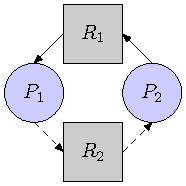
\includegraphics{figures/resource_allocation_safe.pdf}
                        \caption{Safe State}
                    \end{subfigure}%
                    \begin{subfigure}{0.5\linewidth}
                        \centering
                        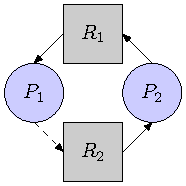
\includegraphics{figures/resource_allocation_unsafe.pdf}
                        \caption{Unsafe State}
                    \end{subfigure}
                    \caption{Resource Allocation Graph States}
                \end{figure}
            The request can be granted only if converting the request edge to an assignment edge does not result 
            in the formation of a cycle in the resource allocation graph.
        \section{Banker's Algorithm}
            Used for multiple instances of resources, where each process must a priori claim the maximum number of resources.
            When a process requests a resource it may have to wait. When a process gets all of its resources, it must return them
            in a finite amount of time.
            \subsection{Data Structures}
                With n processes and m resource types, the following data structures are used
                \begin{itemize}
                    \item \textbf{Available} - Vector of length m. If \textit{available[j]} = k,
                    there are k instances of resource type $R_j$ available.
                    \item \textbf{Max} - $n\times m$ matrix. If \textit{Max[i,j]} = k, then process $P_i$ may
                    request at most k instances of resource type $R_j$.
                    \item \textbf{Allocation} - $n\times m$ matrix. If \textit{Allocation[i,j]} = k, then
                    process $P_i$ is currently allocated k instances of $R_j$.
                    \item \textbf{Need} - $n\times m$ matrix. If \textit{Need[i,j]} = k, then process $P_i$
                    may need k more instances of $R_j$ to complete its task.
                \end{itemize}
                \begin{center}
                    \textit{Need[i,j]} = \textit{Max[i,j]} - \textit{Allocation[i,j]}
                \end{center}
            \subsection{Safety Algorithm}
                \begin{enumerate}
                    \item Letting \textbf{Work} and \textbf{Finish} be vectors of length m and n respectively.
                    \item Initialising \textbf{Work} = \textbf{Available} and \textbf{Finish[i]} = false for $i = 0,1,...,n-1$
                    \item Find an \textbf{i} such that \textbf{Finish[i] = false} and \textbf{Need$\leq$Work}
                        \subitem If no such \textbf{i} exists, go to step 4
                    \item \textbf{Work = Work + Allocation[i]}, \textbf{Finish[i] = true}
                        \subitem Go to step 2
                    \item If \textbf{Finish[i] = true} for all \textbf{i}, the system is in a safe state.
                \end{enumerate}
            \subsection{Resource-Request Algorithm for Process $P_i$}
                \textbf{Request[i]} = request vector for process $P_i$. If \textbf{Request[i,j] = k}, then process
                $P_i$ wants k instances of resource type $R_j$.\\
                \begin{enumerate}
                    \item if \textbf{Request[i]} $\leq$ \textbf{Need[i]}, go to step 2. Otherwise, raise error condition
                    since process has exceeded its maxmimum claim.
                    \item if \textbf{Request[i]} $\leq$ \textbf{Available}, go to step 3. Otherwise, $P_i$ must wait as
                    resources are unavailable.
                    \item Pretend to allocate the requested resources to $P_i$ by modifying the state as follows
                        \begin{center}
                            \textbf{Available = Available - Request}\\
                            \textbf{Allocation[i] = Allocation[i] - Request[i]}\\
                            \textbf{Need[i] = Need[i] - Request[i]}\\
                        \end{center}
                        \begin{itemize}
                            \item If safe state, then resources will be allocated to $P_i$
                            \item If unsafe state, $P_i$ must wait, and the old resource-allocation state will be stored
                        \end{itemize}
                \end{enumerate}
            \subsection{Example}
                Given 4 processes [$P_0, P_1, P_2, P_3, P_4$] and 3 resource types [A (10 instances), B (5 instances), C (7 instances)].\\
                At time $t_0$, the following snapshot of the system has been taken\\
                \begin{center}
                    \begin{tabular}{cccc}
                        & Allocation & Max & Available\\
                        \toprule
                        & A B C & A B C & A B C\\
                        $P_0$ & 0 1 0 & 7 5 3 & 3 3 2\\
                        $P_1$ & 2 0 0 & 3 2 2 & \\
                        $P_2$ & 3 0 2 & 9 0 2 & \\
                        $P_3$ & 2 1 1 & 2 2 2 & \\
                        $P_4$ & 0 0 2 & 4 3 3 & \\
                        \bottomrule
                    \end{tabular}
                \end{center}
                The content of matrix \textbf{Need} is calculated as follows
                \begin{center}
                    \begin{tabular}{cccc}
                        & Allocation & Max & Need\\
                        \toprule
                        & A B C & A B C & A B C\\
                        $P_0$ & 0 1 0 & 7 5 3 & 7 4 3\\
                        $P_1$ & 2 0 0 & 3 2 2 & 1 2 2\\
                        $P_2$ & 3 0 2 & 9 0 2 & 6 0 0\\
                        $P_3$ & 2 1 1 & 2 2 2 & 0 1 1\\
                        $P_4$ & 0 0 2 & 4 3 3 & 4 3 1\\
                        \bottomrule
                    \end{tabular}
                \end{center}
                This system is in a safe state since the sequence $<$ $P_1$, $P_3$, $P_4$, $P_0$, $P_2$ $>$ satisfies the safety algorithm.\\
    \chapter{File Systems and Protection}
        \section{Protection}
            \subsection{Goals of Protection}
                In one protection model, the computer consists of a collection of objects, hardware and/or software, where each object has a unique
                name and can be accessed through a well-defined set of operations.\\
                The protection problem is to ensure that each object is accessed correctly and only by the processes that are allowed to do so.
            \subsection{Principles of Protection}
                The guiding principle of protection is the \textcolor{blue}{principle of least privilege}, where;
                \begin{itemize}
                    \item Programs, users, and systems should be given just enough the privileges to perform their tasks
                    \item Limits damage if process is compromised
                    \item Can be static (during system or process lifetime) or dynamic (changed by process as needed) \textcolor{blue}{domain switching,
                    privilege escalation}
                    \item "Need to know" is a similar concept regarding access to data.
                \end{itemize}
                The \textcolor{blue}{grain} aspect
                \begin{itemize}
                    \item Rough-grained privilege management - easier, simpler, but less privilege levels as they are done in chunks
                        \subitem Processes either have all privileges of user or of root
                    \item Fine-grained management - more complex, more overhead, but more stringent and protective
                        \subitem File ACL Lists, RBAC
                \end{itemize}
            \subsection{Domain of Protection}
                Protection rings seperate functions into domains and order them hierarchically. A generalization of rings is using 
                domains without a hierarchy.\\
                A computer system can be treated as a collection of processes and objects.\\
                Objects in this context can be hardware or software entities.\\
                \subsubsection{Domain Structure}
                    In order to facilitate this scheme, a process may operate within a \textcolor{blue}{protection domain} which 
                    specifices the resources that the process may access.\\
                    Each domain defines a set of objects and the types of operations that may be invoked.\\
                    The ability to execute an operation on an object is an \textcolor{blue}{access right}.\\
                    A domain is a collection of access rights, each an ordered pair
                    \begin{center}
                        \textbf{(object, set of operations)}
                    \end{center}
                    For example, if domain $D_1$ has access rights \textbf{(file \textit{F}, read, write)}, then process $P_1$ in domain $D_1$
                    may read and write \textit{F}.\\
                    Domains may share access rights as well, for example, if domain $D_2$ has access rights \textbf{(file \textit{F}, read)},
                    then process $P_2$ in domain $D_2$ may read \textit{F}.\\ 
                    The association between a process and a domian may be either \textcolor{blue}{static} or \textcolor{blue}{dynamic}.\\
                    Establishing dynamic protection domains is more complex as it involves \textcolor{blue}{domain switching}, where 
                    the process switches from one domain to another.\\
                    \begin{figure}[H]
                        \centering
                        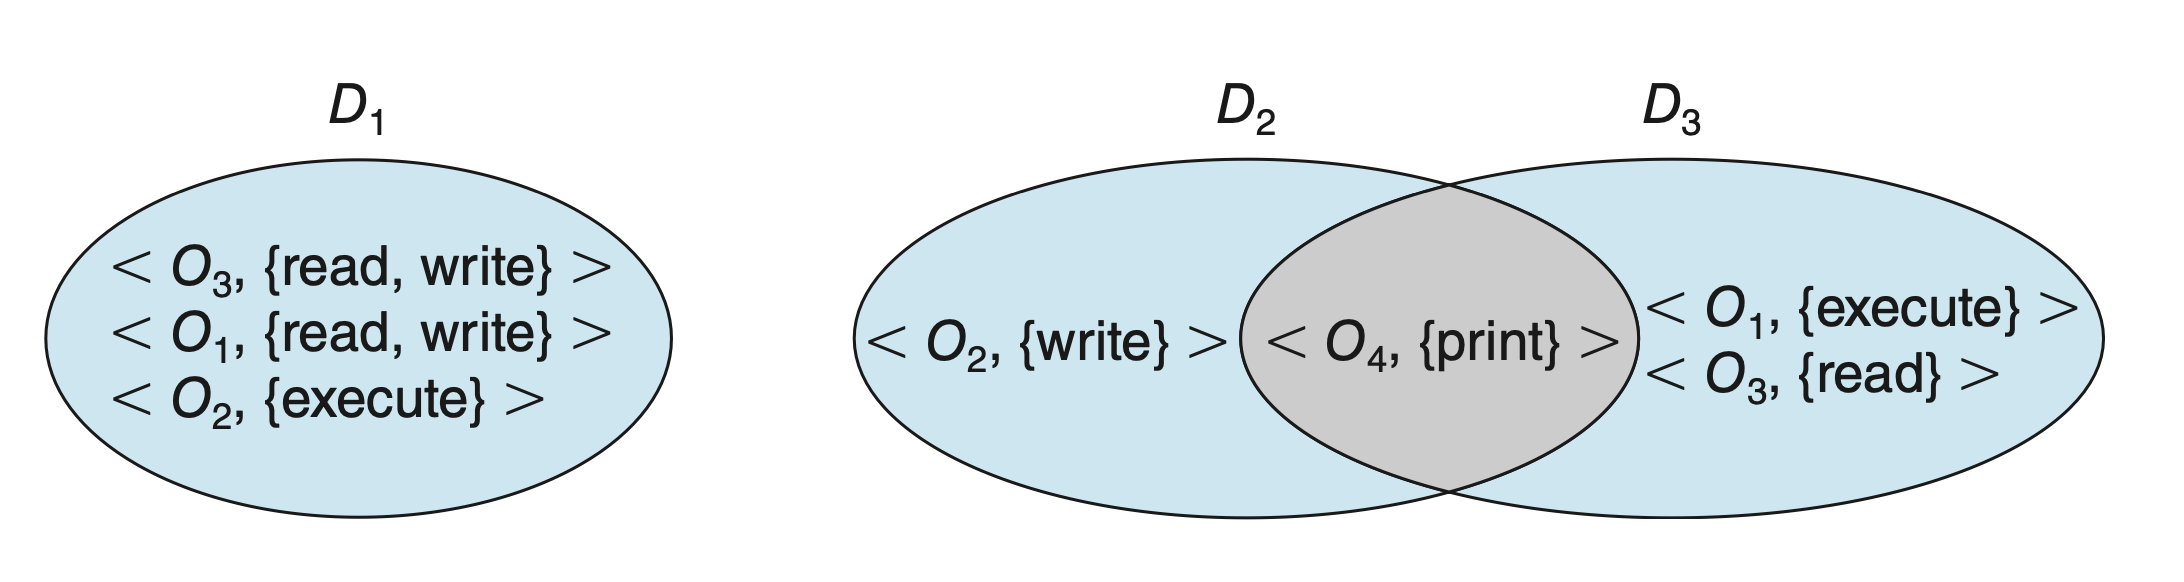
\includegraphics[width=0.6\linewidth]{figures/protection_domains_3.png}
                        \caption{System with three protection domains}
                    \end{figure}
                    Domains can be realised in multiple ways
                    \begin{enumerate}
                        \item Each \textit{user} may be a domain. In this case, the set of objects that can be accessed depends on the identity of the 
                        user. Domain switching occurs when the user is changed (login, su, etc.)
                        \item Each \textit{process} may be a domain. In this case the set of objects that can be accessed depends on the identity of the
                        process. Domain switching occurs when one process sends a message to another process and waits for a response.
                        \item Each \textit{procedure} may be a domain. In this case the set of objects that can be accessed corresponds to the local variables
                        defined within the procedure. Domain switching occurs when a procedure is called.
                    \end{enumerate}
            \subsection{Access Matrix}
                The general model of protection can be viewed abstractly as a matrix, called an \textcolor{blue}{access matrix}. \\
                Rows represent domains, and columns represent objects.\\
                Each entry contains a set of access rights where the entry \texttt{access}(\textit{i,j}) defines the set of operations 
                that a process in domain $D_i$ can invoke on object $O_j$.\\
                \begin{figure}[H]
                    \centering
                    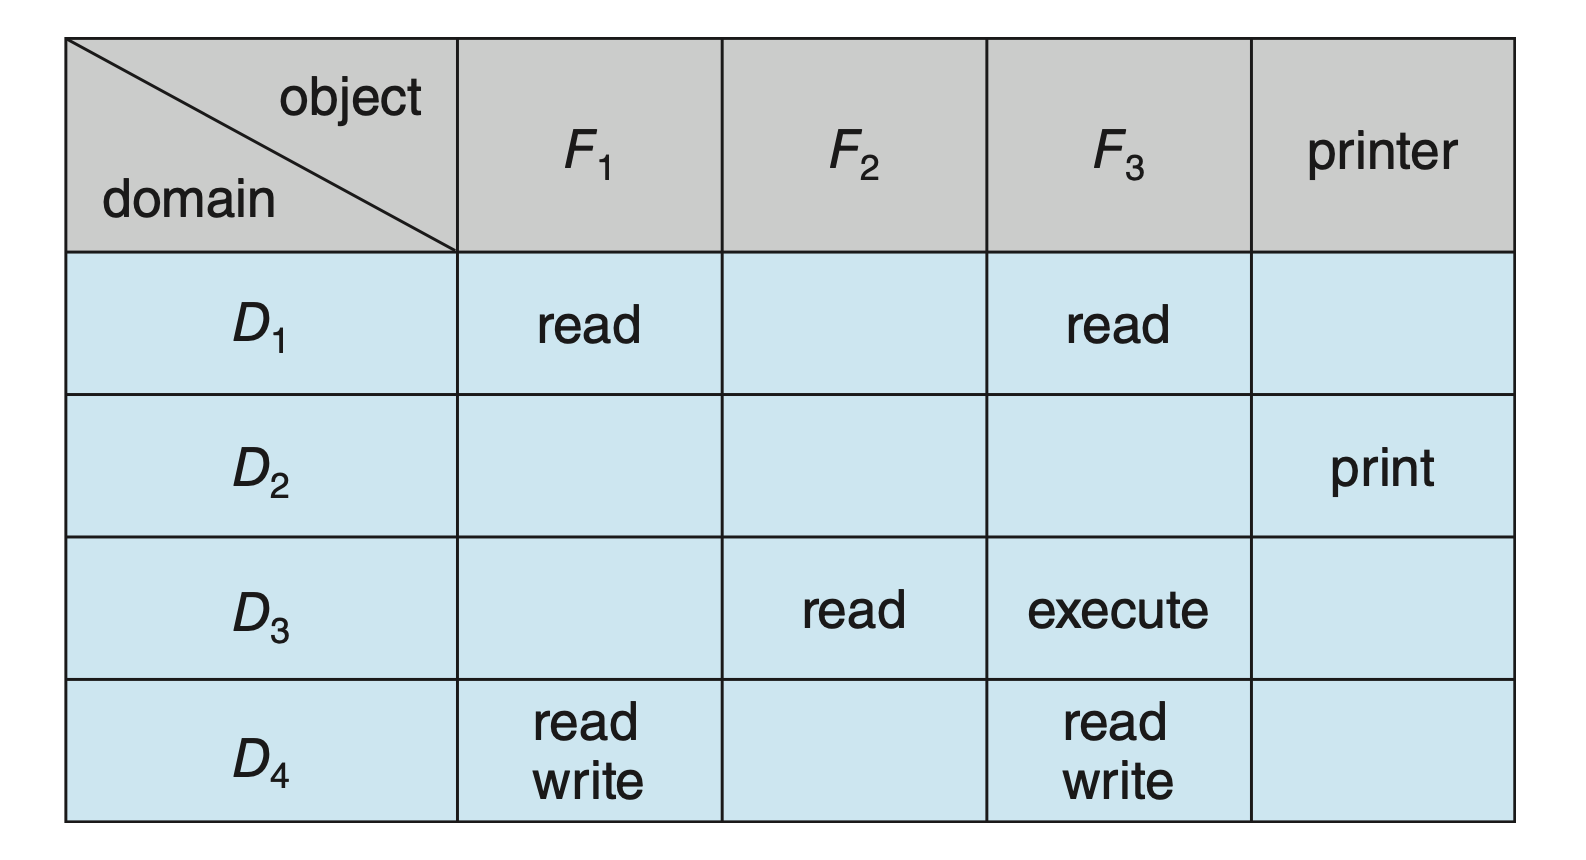
\includegraphics[width=0.6\linewidth]{figures/access_matrix.png}
                    \caption{Access Matrix}
                \end{figure}
                The creator of the object dictates the access column for the object.\\
                Can be expanded to dynamic protection
                \begin{itemize}
                    \item Operations to add, delete rights (columns)
                    \item Special access rights\\
                    \begin{tabular}{ll}
                        -- Owner & of $O_i$ \\
                        -- Copy op & from $O_i$ to $O_j$ (denoted by *) \\
                        -- Control & $D_i$ can modify $D_j$ access rights \\
                        -- Transfer & switch domain from $D_i$ to $D_j$ \\
                    \end{tabular}
                \end{itemize}
                Note that copy and owner are applicable to an object while control and transfer are applicable to a domain.\\
                \begin{figure}[H]
                    \centering
                    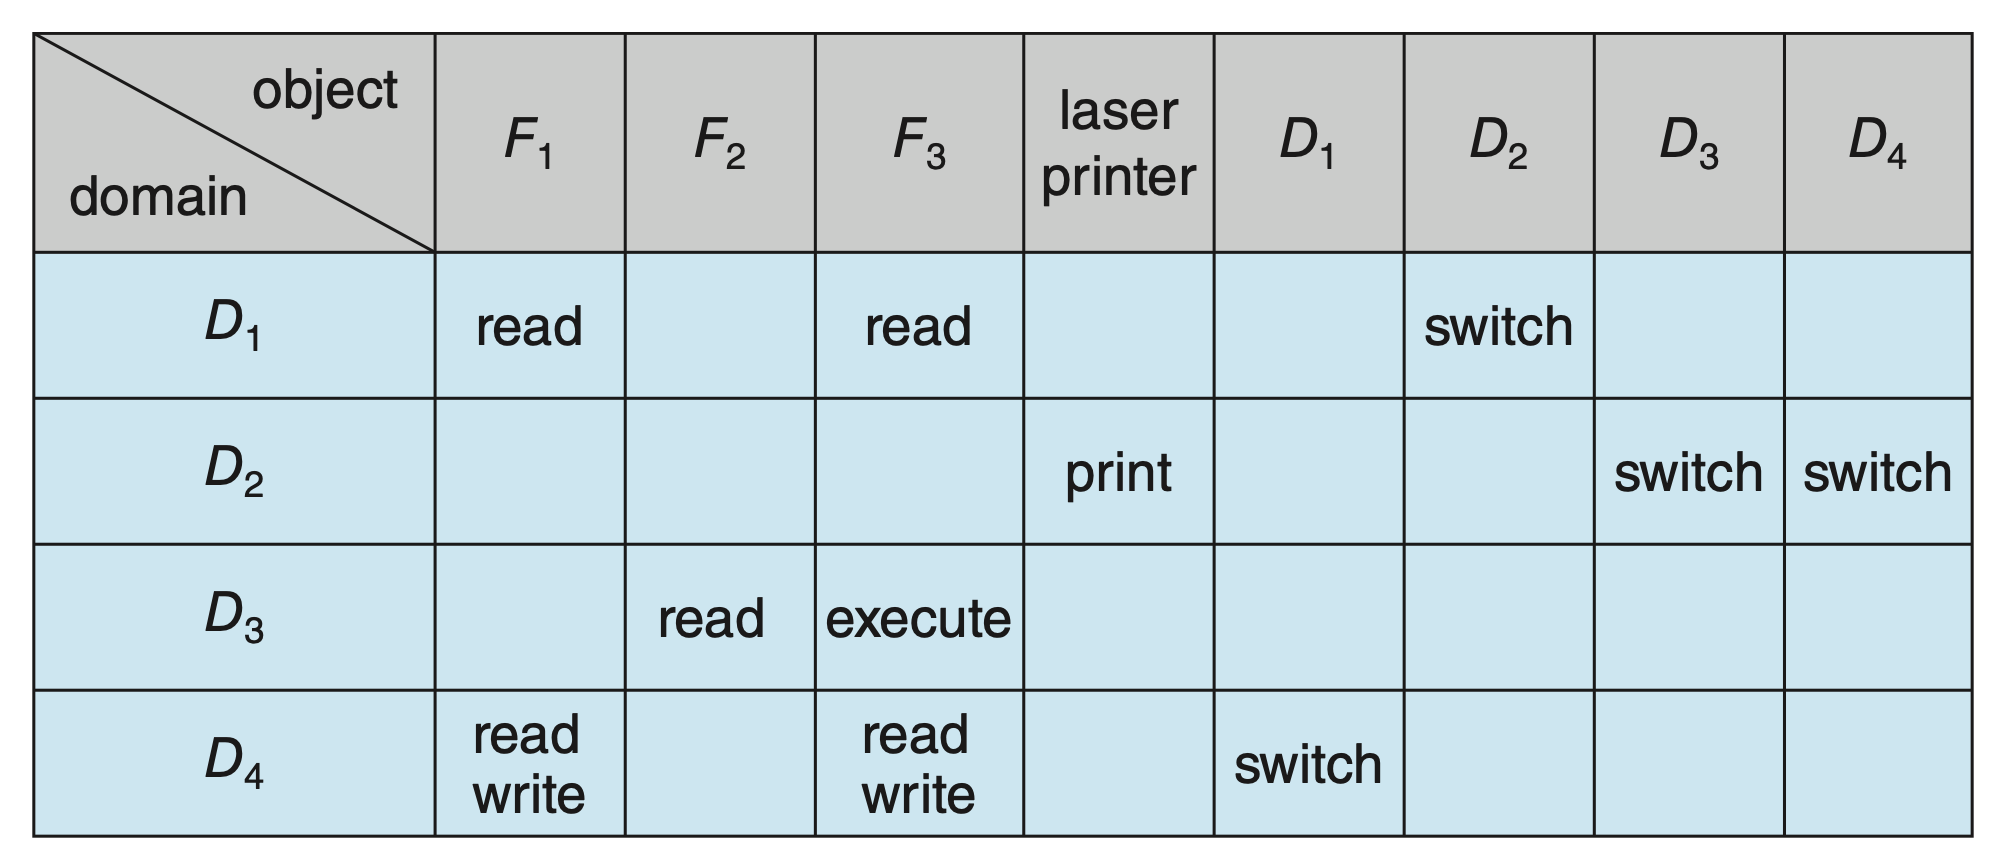
\includegraphics[width=0.6\linewidth]{figures/access_matrix_domobj.png}
                    \caption{Access Matrix with Domains as Objects}
                \end{figure}
                This has the two variants;
                \begin{itemize}
                    \item A right is copied from \texttt{access}(\textit{i,j}) to \texttt{access}(\textit{k,j}).
                    It is then removed from from \texttt{access}(\textit{i,j}). Therefore, is a transfer not a copy.
                    \item Propogation of \texttt{copy} right may be limited. That is, when the right \textit{R*} is
                    copied from \texttt{access}(\textit{i,j}) to \texttt{access}(\textit{k,j}), only the right 
                    \textit{R} (not \textit{R*}) is created. A process executing in domain $D_k$ cannot further copy the right \textit{R}.
                \end{itemize}
                \begin{figure}[H]
                    \centering
                    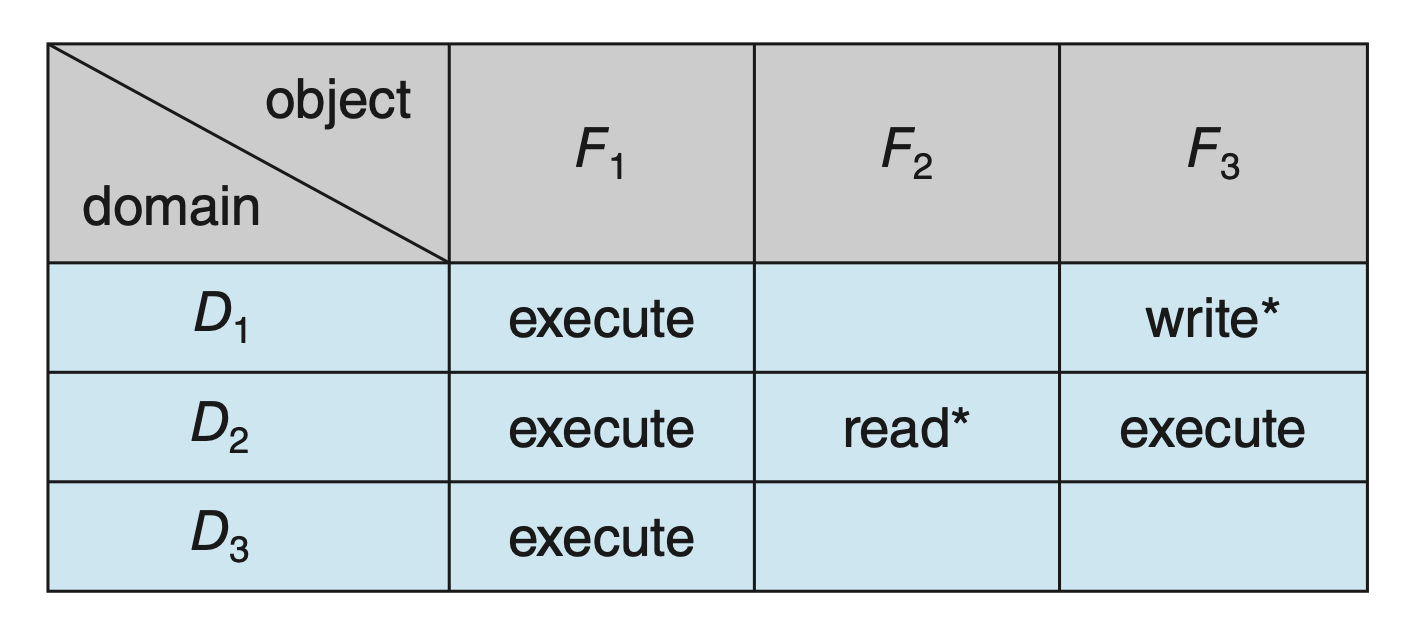
\includegraphics[width=0.4\linewidth]{figures/access_matrix_copy_1.png}%
                    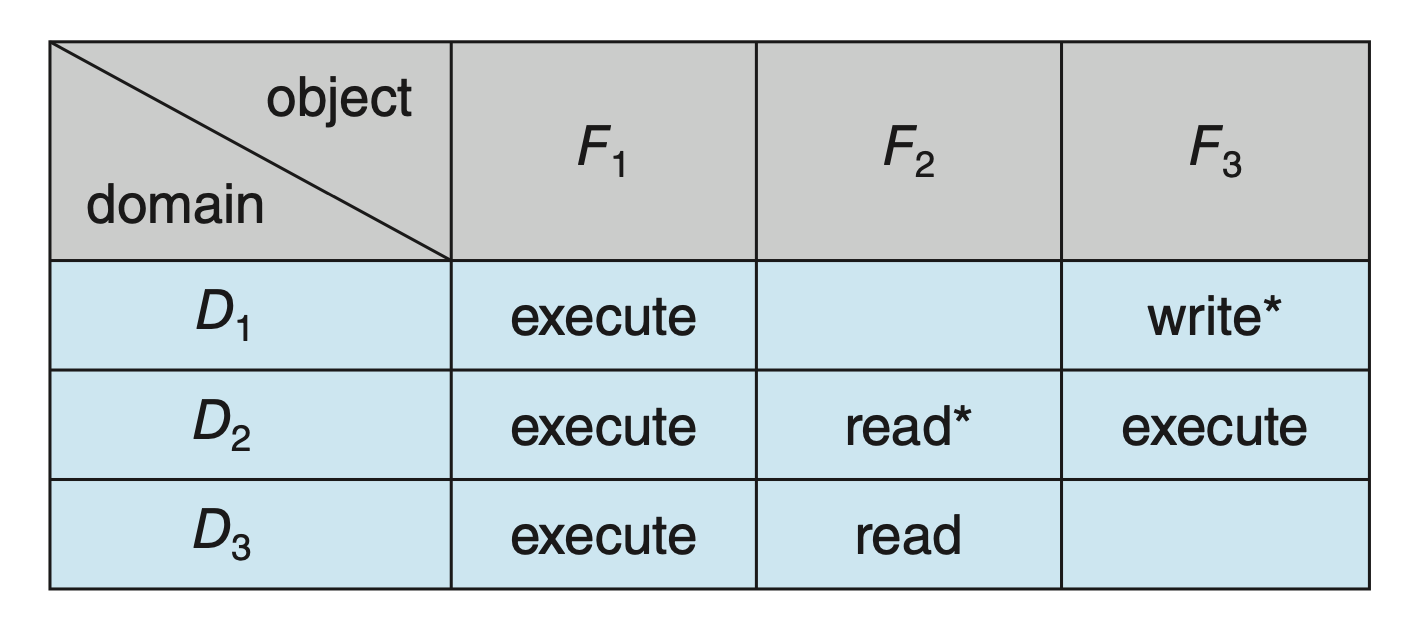
\includegraphics[width=0.4\linewidth]{figures/access_matrix_copy_2.png}
                    \caption{Access Matrix with Copy Rights}
                \end{figure}
            \subsection{Access Control}
                Protection can also be applied to non file resources.\\
                Oracle Solaris 10 provides \textcolor{blue}{role-based access control} (\textcolor{blue}{RBAC})
                to implement least privilege.\\
                \begin{itemize}
                    \item \textbf{Privilege} is the right to execute a system call or use an option within a system call
                    \item Can be assigned to processes
                    \item Users assigned \textbf{roles} granting access to privileges and programs
                        \subitem Enable role via password to gain privileges
                    \item Similar to an access matrix
                \end{itemize}
        \section{File System Interface}
            \subsection{File Concept}
                A file is a named collection of related information that is recorded on secondary storage.
                A logical storage unit that is independent from the physical properties of its storage device.
                From a user's perspective, a file is the smallest allotment of logical secondary storage (data cannot
                be written to secondary storage unless they are within a file).\\
                File types include
                \begin{itemize}
                    \item Data
                        \begin{itemize}
                            \item Numeric
                            \item Character
                            \item Binary
                        \end{itemize}
                    \item Program
                \end{itemize}
                Some files (plain text) do not have formatting while some do.\\
                In general, a file is a sequence of bits, bytes, lines, or records
                \subsubsection{File Attributes}
                    File attributes vary between operating systems, but in general consist of 
                    \begin{itemize}
                        \item \textbf{Name} - only information that is kept in human readable form
                        \item \textbf{Identifier} - unique tag (number) that identifies file within system
                        \item \textbf{Type} - needed for systems that support different types
                        \item \textbf{Location} - pointer to file location on device
                        \item \textbf{Size} - current size
                        \item \textbf{Protection} - controls read, write and execute privileges
                        \item \textbf{Time, data, and user identification} - data for protection, security, and usage monitoring
                    \end{itemize}
                    Information about files are kept in the directory structure, which is maintained on secondary storage.
                \subsubsection{File Operations}
                    Files are an \textbf{abstract data type} with the following defined operations
                    \begin{itemize}
                        \item \textbf{Create}
                            \subitem Find space in the file system and then add an entry of the new file into the directory.
                        \item \textbf{Write}
                            \subitem The file system searches the directory to find the file's writing location, writes to that location,
                            then updates the write pointer.
                        \item \textbf{Read}
                            \subitem The file system searches the directory to find the file's read location, reads from that
                            location and then updates the read pointer.
                        \item \textbf{Reposition}
                            \subitem The file system searches the directory to find the file's location, then updates the read
                            and write pointers.
                        \item \textbf{Delete}
                            \subitem The file system searches the directory to find the file's location, then removes the file 
                            from the directory and marks the space as available.
                        \item \textbf{Truncate}
                            \subitem The file system searches the directory to find the file's location, then removes the file 
                            from the directory and marks the space as available. The file system then updates the file's size 
                            attribute.
                    \end{itemize}
                    These primitive operatiosn can then be combined to perform other file operations (can create a file copy operation
                    by creating a new file and then reading from the old and writing to the new)
                    \begin{itemize}
                        \item \textbf{Open}$(F_i)$ 
                            \subitem Searches the directroy structure on disk for entry $F_i$ and moves the content of the entry 
                            into internal system table. The entry contains information about the location of the file, its size, 
                            and other attributes. The system also allocates resources to manage the open file table. 
                        \item \textbf{Close}$(F_i)$
                            \subitem Writes any cached information belonging to $F_i$ to disk, removes $F_i$ from the open file table, 
                            and frees up any table space allocated to $F_i$ in the system.
                    \end{itemize}
                \subsubsection{Open Files}
                    Several pieces of data are needed to manage open files
                    \begin{itemize}
                        \item \textbf{Open-file table}
                            \subitem Tracks open files
                        \item \textbf{File pointer}
                            \subitem Pointer to last read/write location, per process that has the file open
                        \item \textbf{File-open count}
                            \subitem Counter of the number of times a file is open to allow removal of data from the open-file table
                            when the last process closes it
                        \item \textbf{Disk location}
                            \subitem Cache of data access information
                        \item \textbf{Access rights}
                            \subitem Per process access mode information
                    \end{itemize}
                \subsubsection{Open File Locking}
                    Provied by some operating systems and file systems and is similar to reader-writer locks
                    \begin{itemize}
                        \item \textbf{Shared lock}
                            \subitem Similar to a reader lock. Several processes can acquire concurrently
                        \item \textbf{Exclusive lock}
                            \subitem Similar to a writer lock. Only one process can acquire at a time
                    \end{itemize}
                    Mandatory or Advisory
                    \begin{itemize}
                        \item \textbf{Mandatory}
                            \subitem Access is denied depending on the locks held and requested
                        \item \textbf{Advisory}
                            \subitem Processes can find status of locks and decide what to do
                    \end{itemize}
                \subsubsection{File Structure}
                    File types can be used to indicate the internal structure of a file where an empty type
                    menas a sequence of words/bytes.\\
                    Simple record structure
                    \begin{itemize}
                        \item Lines
                        \item Fixed length
                        \item Variable length
                    \end{itemize}
                    Complex structures
                    \begin{itemize}
                        \item Formatted document
                        \item Relocatable load file
                    \end{itemize}
                    If the operating system suports a file type, it needs to contain the code to support that file structure.
                    Some operating systems (Unix, Windows) impose a minimal number of structures.
                    \subitem Example: Unix considers each file to be a sequence of 8-bit types. No interpretation for these 
                    8 bits
            \subsection{Access Methods}
                \begin{itemize}
                    \item \textbf{Sequential Access}
                    % bold listing
                    \begin{minted}{c}
                        read_next(record);
                        write_next(record);
                        reset(); /* Move the file pointer to the beginning of the file */ 
                    \end{minted}
                    \item \textbf{Direct Access}
                    \begin{minted}{c}
                        read(n);
                        write(n);
                        position_to(n); /* Move the file pointer to the nth record */
                        read_next();
                        write_next();
                    \end{minted}
                    n = \textcolor{blue}{relative block number}
                \end{itemize}
                \begin{figure}[H]
                    \centering
                    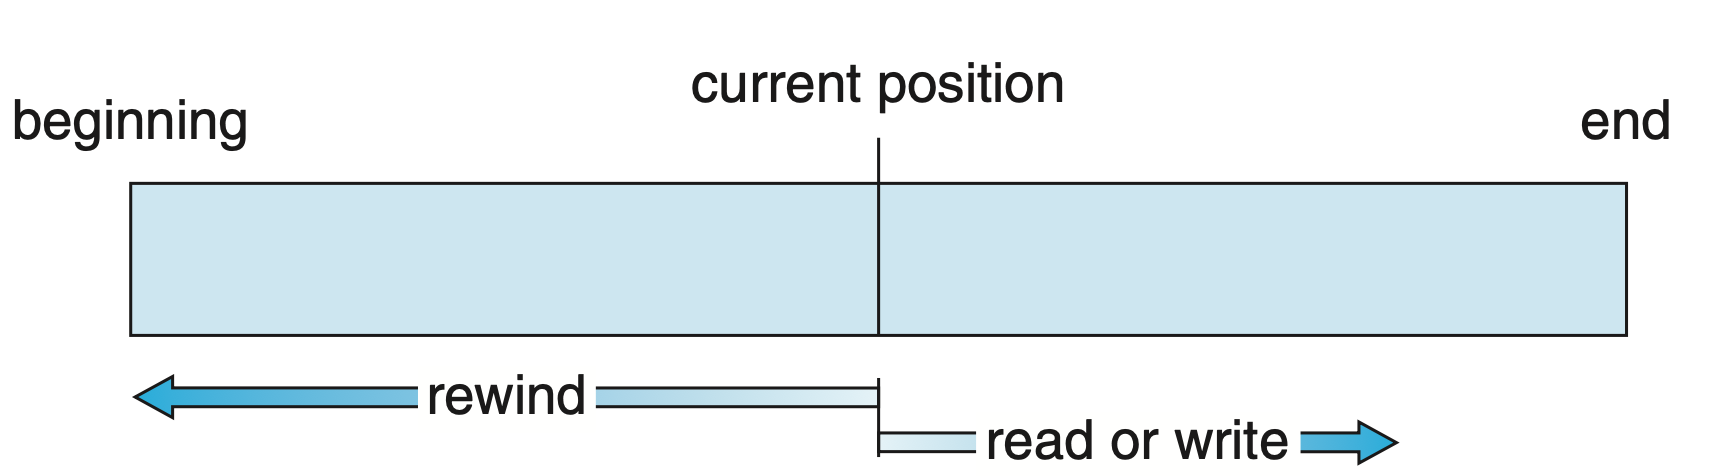
\includegraphics[width=0.6\linewidth]{figures/sequential_access.png}
                    \caption{Sequential Access}
                \end{figure}
                \begin{figure}[H]
                    \centering
                    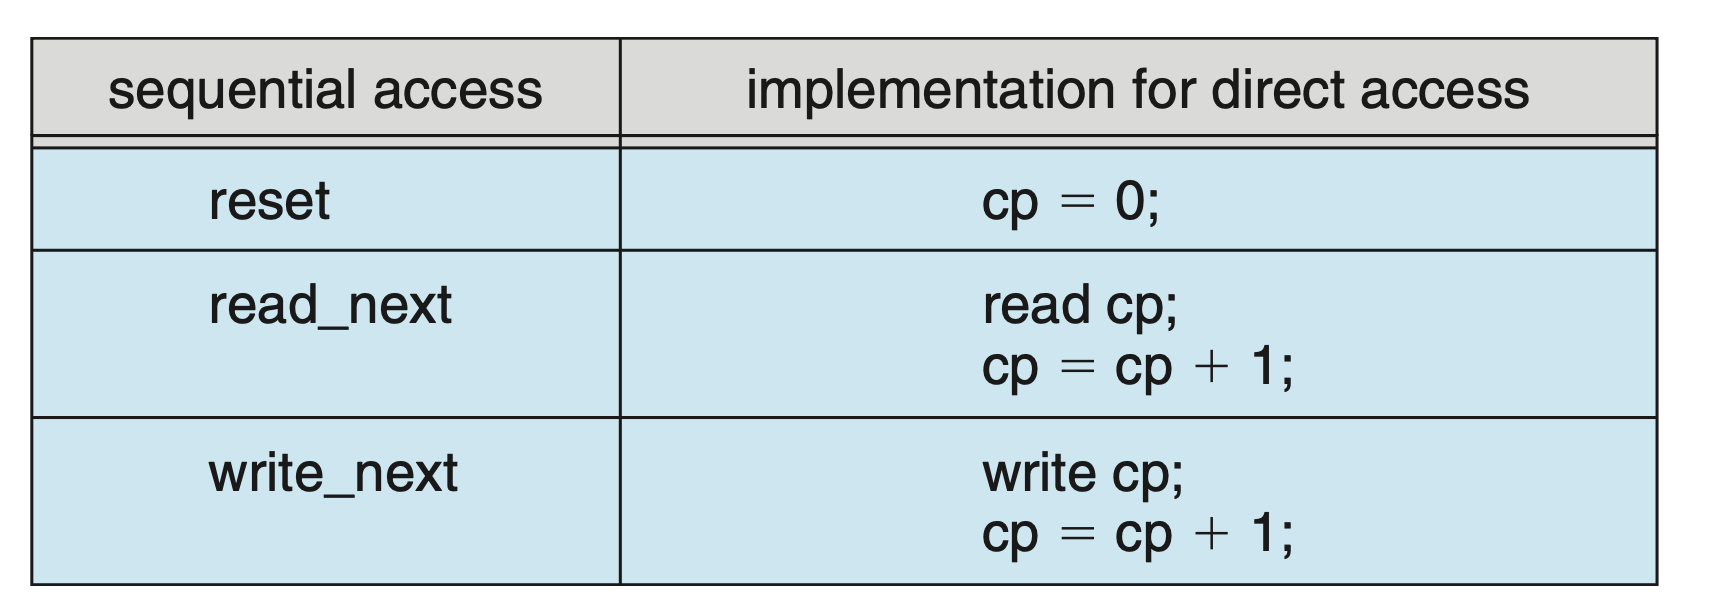
\includegraphics[width=0.6\linewidth]{figures/sequential_access_sim.png}
                    \caption{Simulation of sequential access on a direct access file}
                \end{figure}
                \subsubsection{Other Access Methods}
                    Access methods can be built on top of the direct access method, generally involving the creation of 
                    an \textcolor{blue}{index} for the file. Keeping the index in memory can speed up locating data to be operating
                    on (UP code + record of data about that item). Alternatively, index (in memory) or index (on disk) if
                    space constraints arise.\\
                    IBM Indexed Sequential Access Method (ISAM)\\
                    \begin{itemize}
                        \item Small master index which points to disk blocks of secondary index
                        \item Files are kept sorted on a defined key
                        \item All managed on the operating system
                    \end{itemize}
                    VMS operating system provides index and relative files.
                    \begin{figure}
                        \centering
                        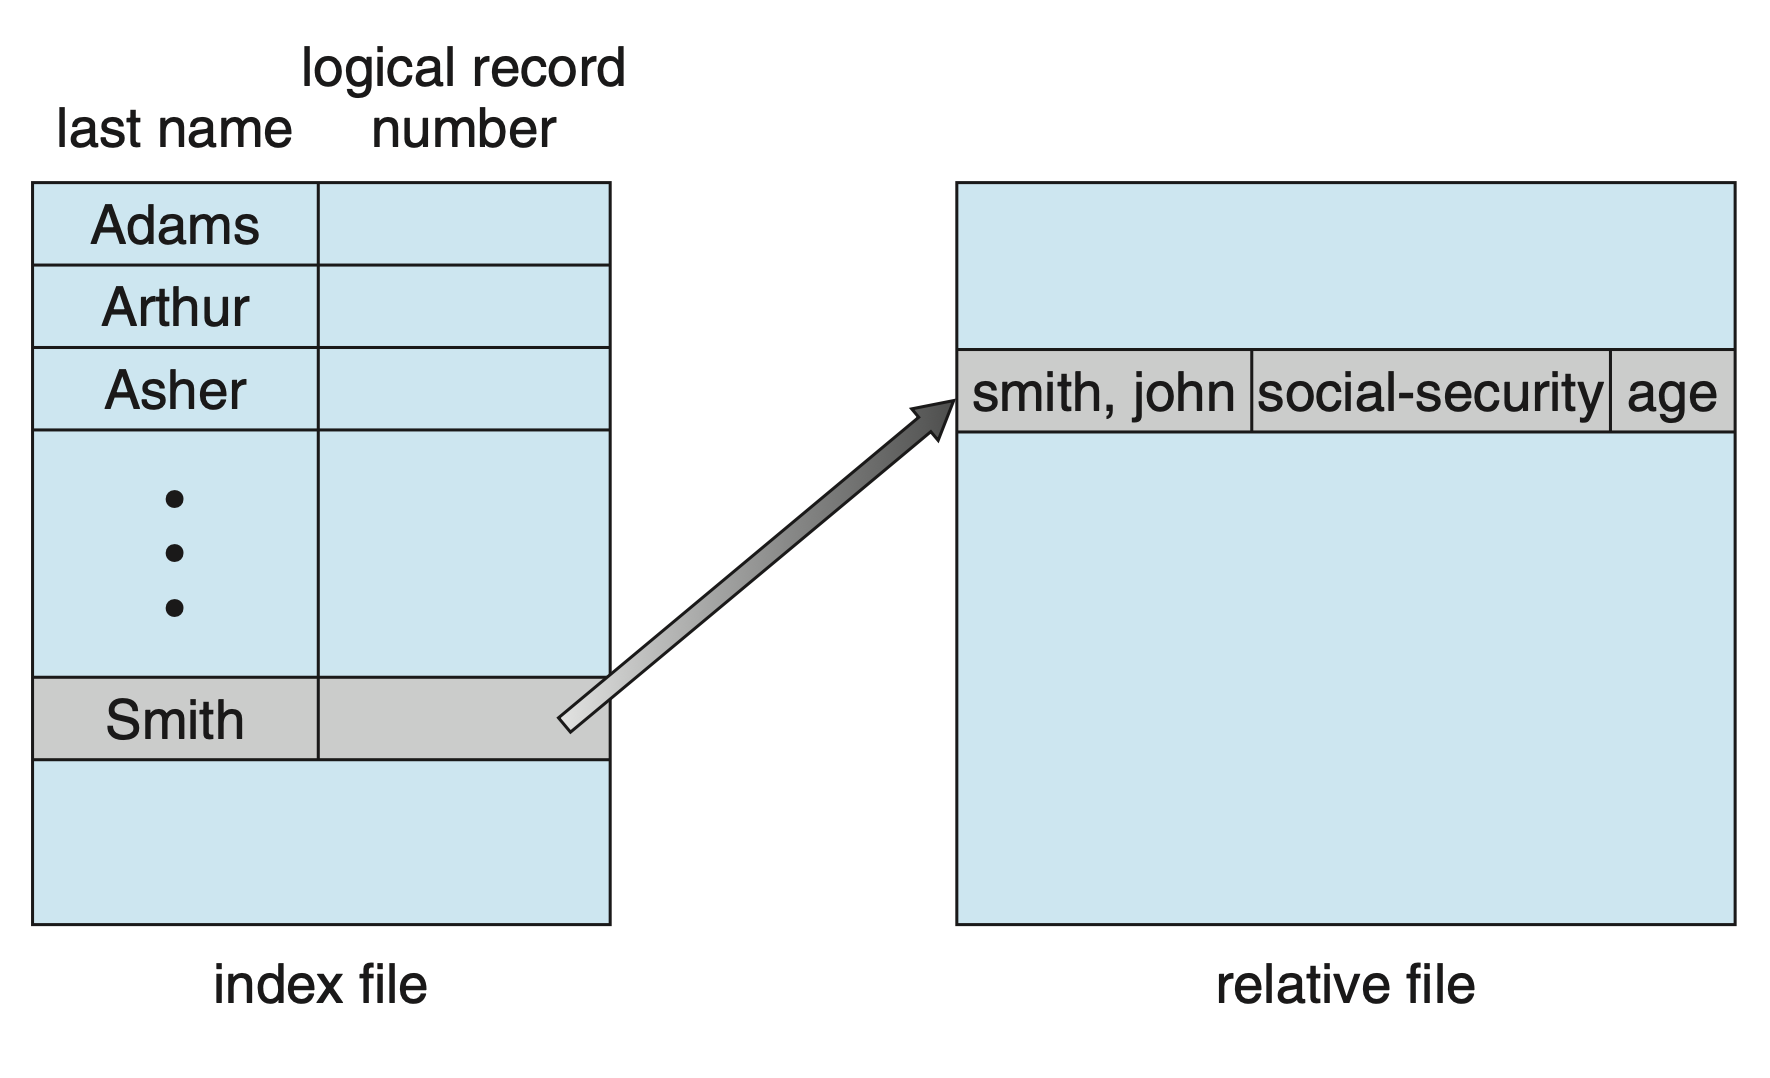
\includegraphics[width=0.6\linewidth]{figures/index_and_relative_files.png}
                    \end{figure}
            \subsection{File-Systems}
                \subsubsection{Directory Structure}
                        Is a collection of nodes containing information about all the files.\\
                        \begin{figure}[H]
                            \centering
                            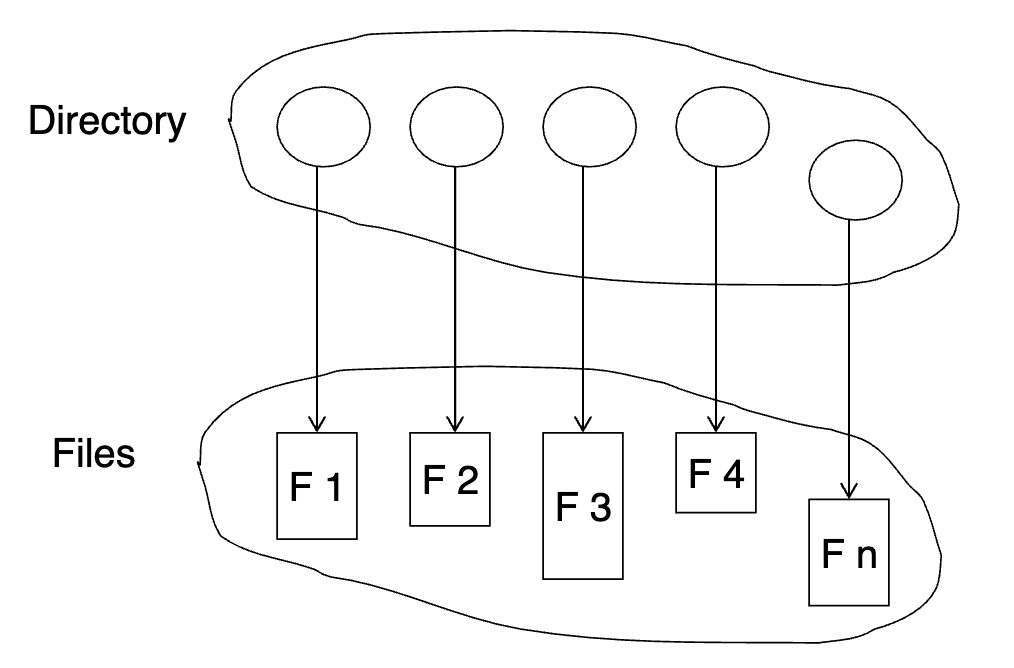
\includegraphics[width=0.6\linewidth]{figures/directory_structure.png}
                            \caption{Directory Structure}
                        \end{figure}
                    \subsubsection{Disk Structure}
                        Disks, can be divided into \textcolor{blue}{partitions}, which can be \textcolor{blue}{RAID}
                        (Redundant Array of Independent Disks) protected against a failure. They can also be used raw,
                        without a file system/not formatting with a file system. Partitions are also called \textcolor{blue}{minidisks, slices}.
                        An entity containing a file system is also called a \textcolor{blue}{volume}, where each volute containing file
                        system also tracks that file system's information in the \textcolor{blue}{device directory} or
                        \textcolor{blue}{volume table of contents}.\\
                        There are special purpose and general purpose file systems.\\
                        Frequently within the same operating system.
                    \subsubsection{Types of File Systems}
                        While we focus on general purpose file systems, there are special file systems used by operating systems
                        as well. For example, with Solaris:
                        \begin{itemize}
                            \item tmpfs
                                \subitem Temporary file system in memory, volatile and fast
                            \item objfs
                                \subitem Interface into kernel memory to get kernel symbols for debugging
                            \item ctfs
                                \subitem Contract file system for managing daemons
                            \item lofs
                                \subitem Loopback file system allowing one filesystem to be accessed in place of another
                            \item procfs
                                \subitem Kernel interface to process structures
                            \item ufs, zfs
                                \subitem General purpose file systems
                        \end{itemize}
                    \subsubsection{File System Mounting}
                        A file system must be mounted before being accessed.\\
                        An unmounted file system is mounted at the mount point
                        \begin{figure}[H]
                            \centering
                            \begin{subfigure}{0.5\linewidth}
                                \centering
                                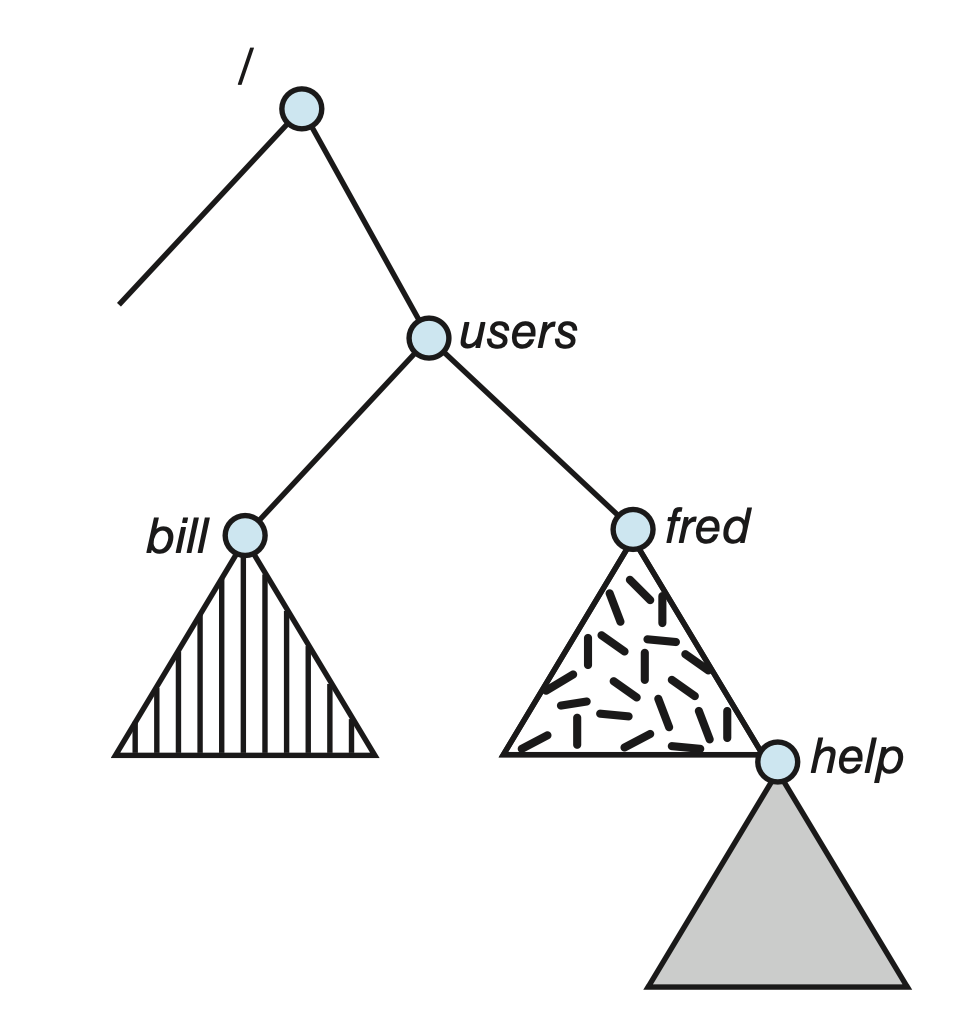
\includegraphics[width=0.6\linewidth]{figures/existing_system.png}
                                \caption{Existing System}
                            \end{subfigure}%
                            \begin{subfigure}{0.5\linewidth}
                                \centering
                                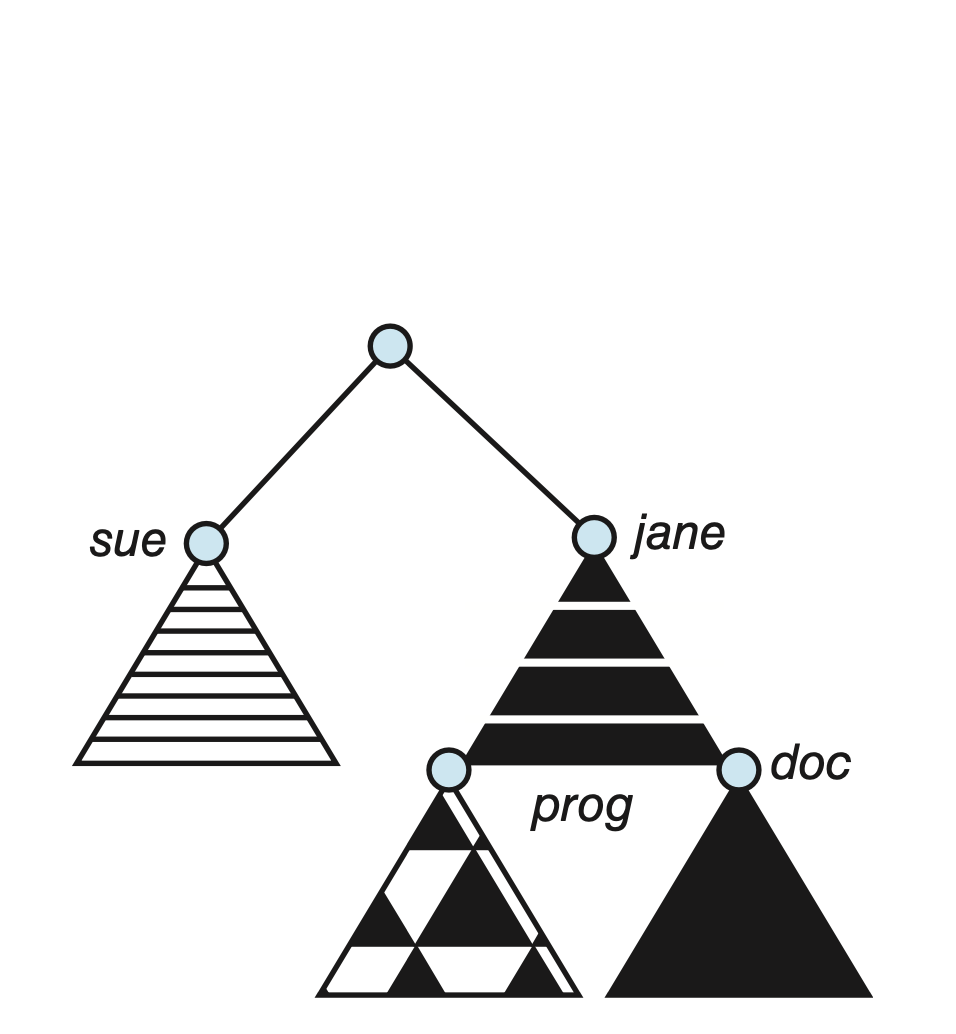
\includegraphics[width=0.6\linewidth]{figures/unmounted_volume.png}
                                \caption{Unmounted Volume}
                            \end{subfigure}
                            \caption{File System Mounting}
                        \end{figure}
                        \begin{figure}[H]
                            \centering
                            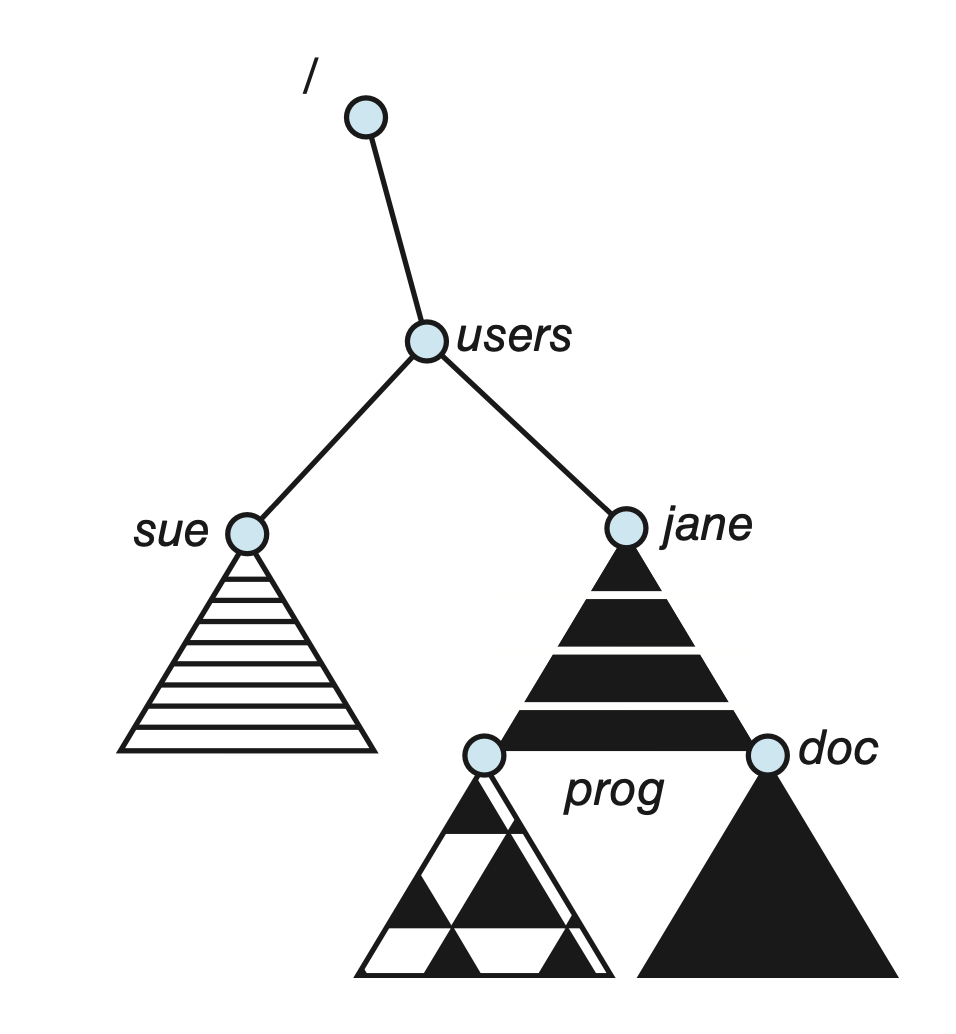
\includegraphics[width=0.3\linewidth]{figures/mounted_volume.png}
                            \caption{Mounted Volume at /users}
                        \end{figure}
                \subsection{Directory Structures}
                    \subsubsection{Operations Performed on Directory}
                            A diretory can be viewed as a data structure that stores information about the files in the directory.
                            The operations that can be performed on a directory are
                            \begin{itemize}
                                \item Search for a file
                                \item Create a file
                                \item Delete a file
                                \item List a directory
                                \item Rename a file
                                \item Traverse the file system
                            \end{itemize}
                    \subsubsection{Single-Level Directory}
                        Simplest directory structure, where a single directory contains all the files on the disk.\\
                        \begin{figure}[H]
                            \centering
                            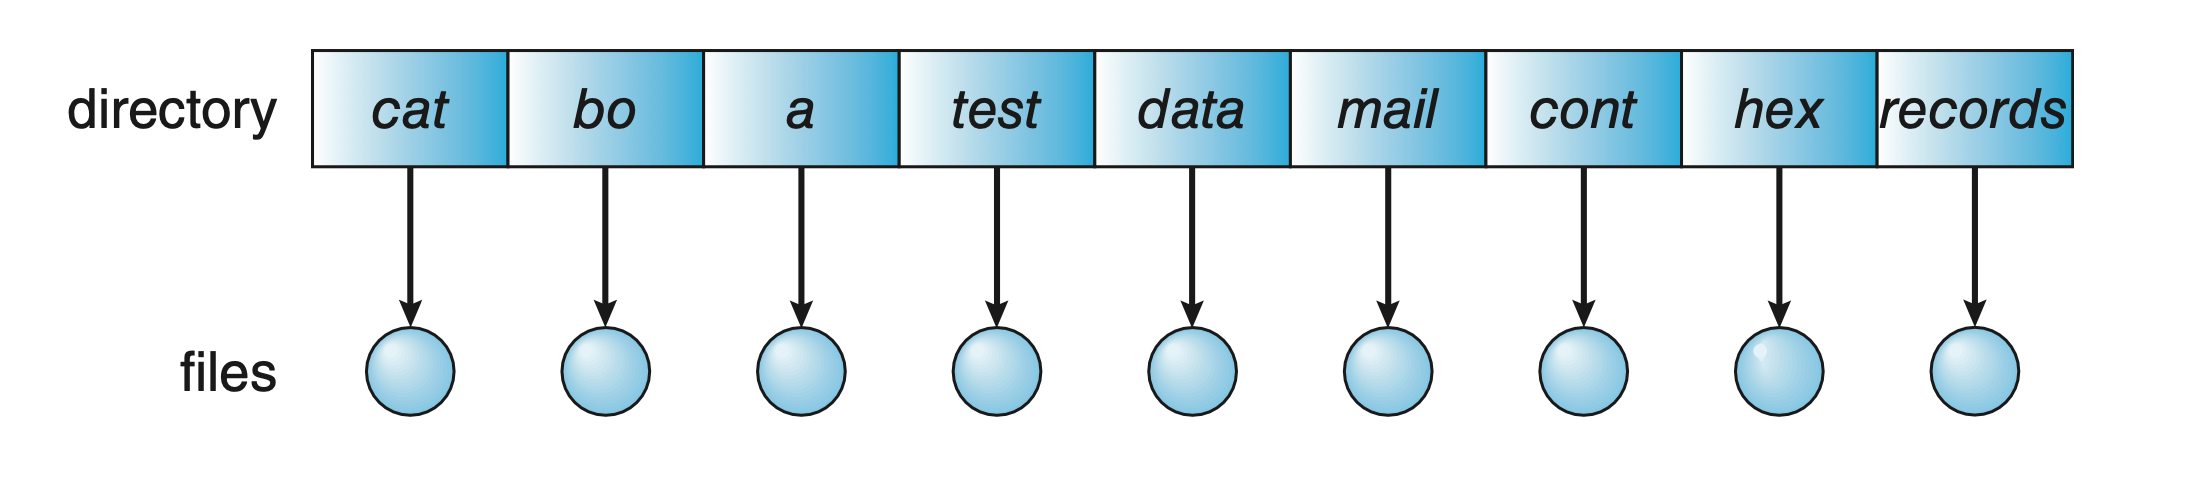
\includegraphics[width=0.6\linewidth]{figures/single_level_dir.png}
                            \caption{Single-Level Directory}
                        \end{figure}
                    \subsubsection{Two-Level Directory}
                        Seperate directory for each user (\textcolor{blue}{user file directory UFD}) and one directory for all users
                        (\textcolor{blue}{master file directory MFD}).\\
                        \begin{figure}[H]
                            \centering
                            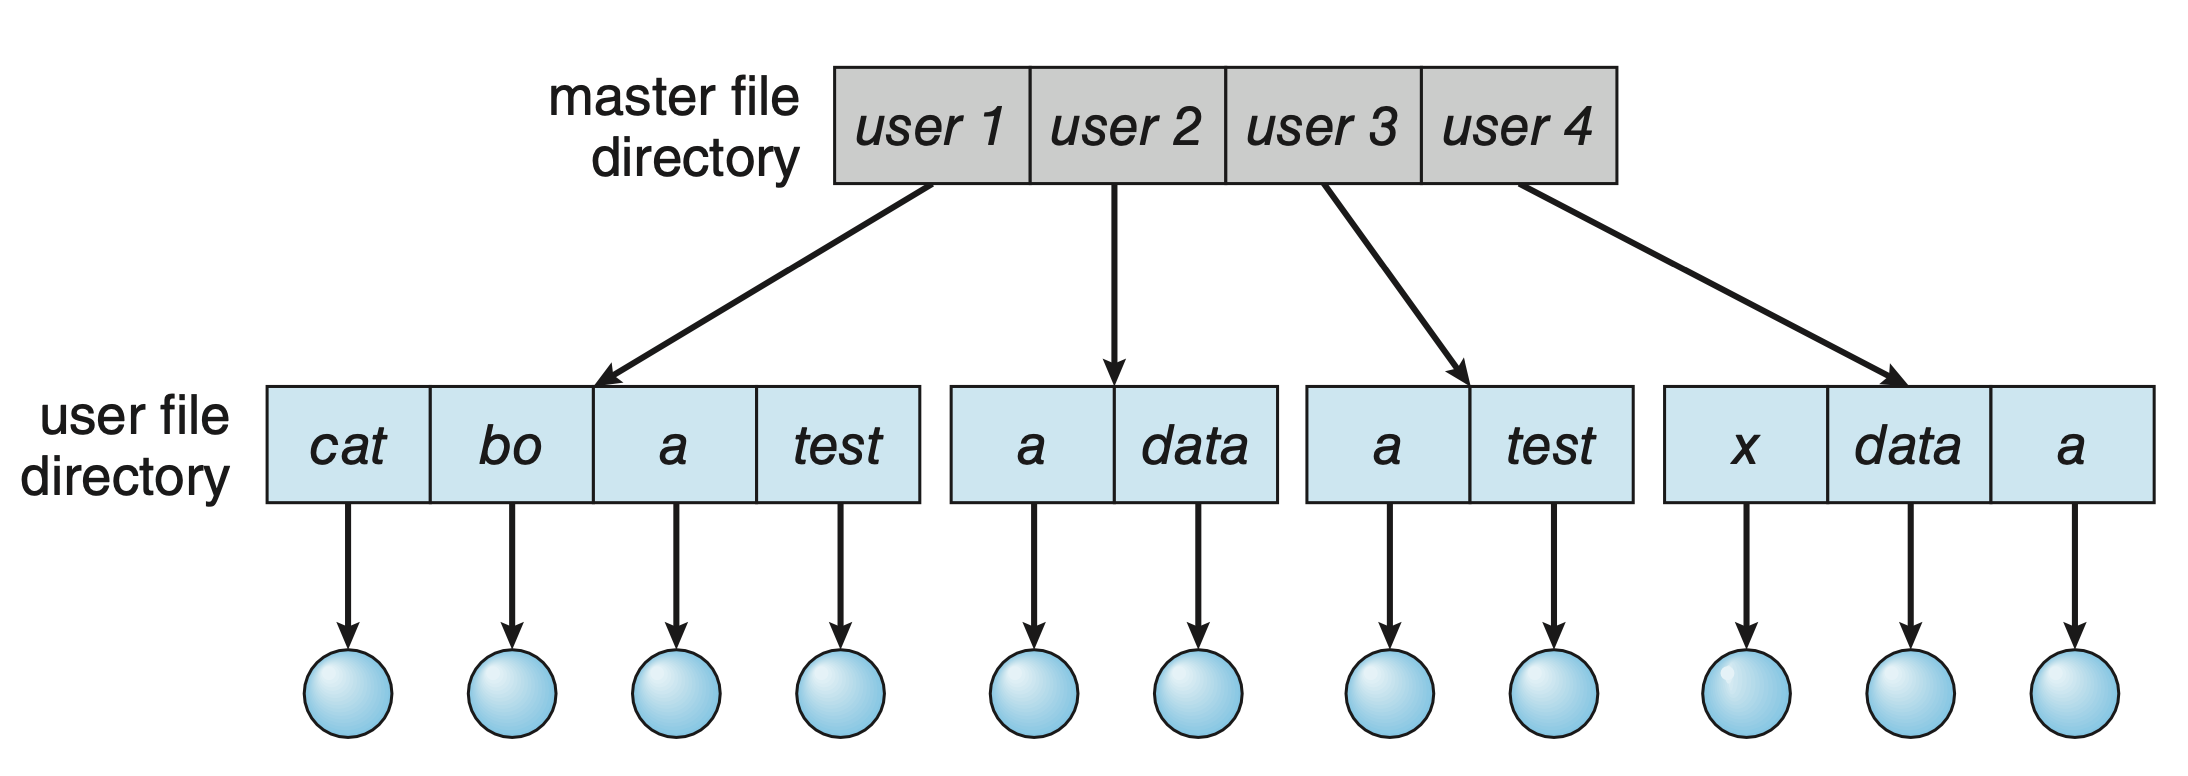
\includegraphics[width=0.6\linewidth]{figures/two_level_dir.png}
                            \caption{Two-Level Directory}
                        \end{figure}
                    \subsubsection{Tree-Structured Directory}
                        \begin{figure}[H]
                            \centering
                            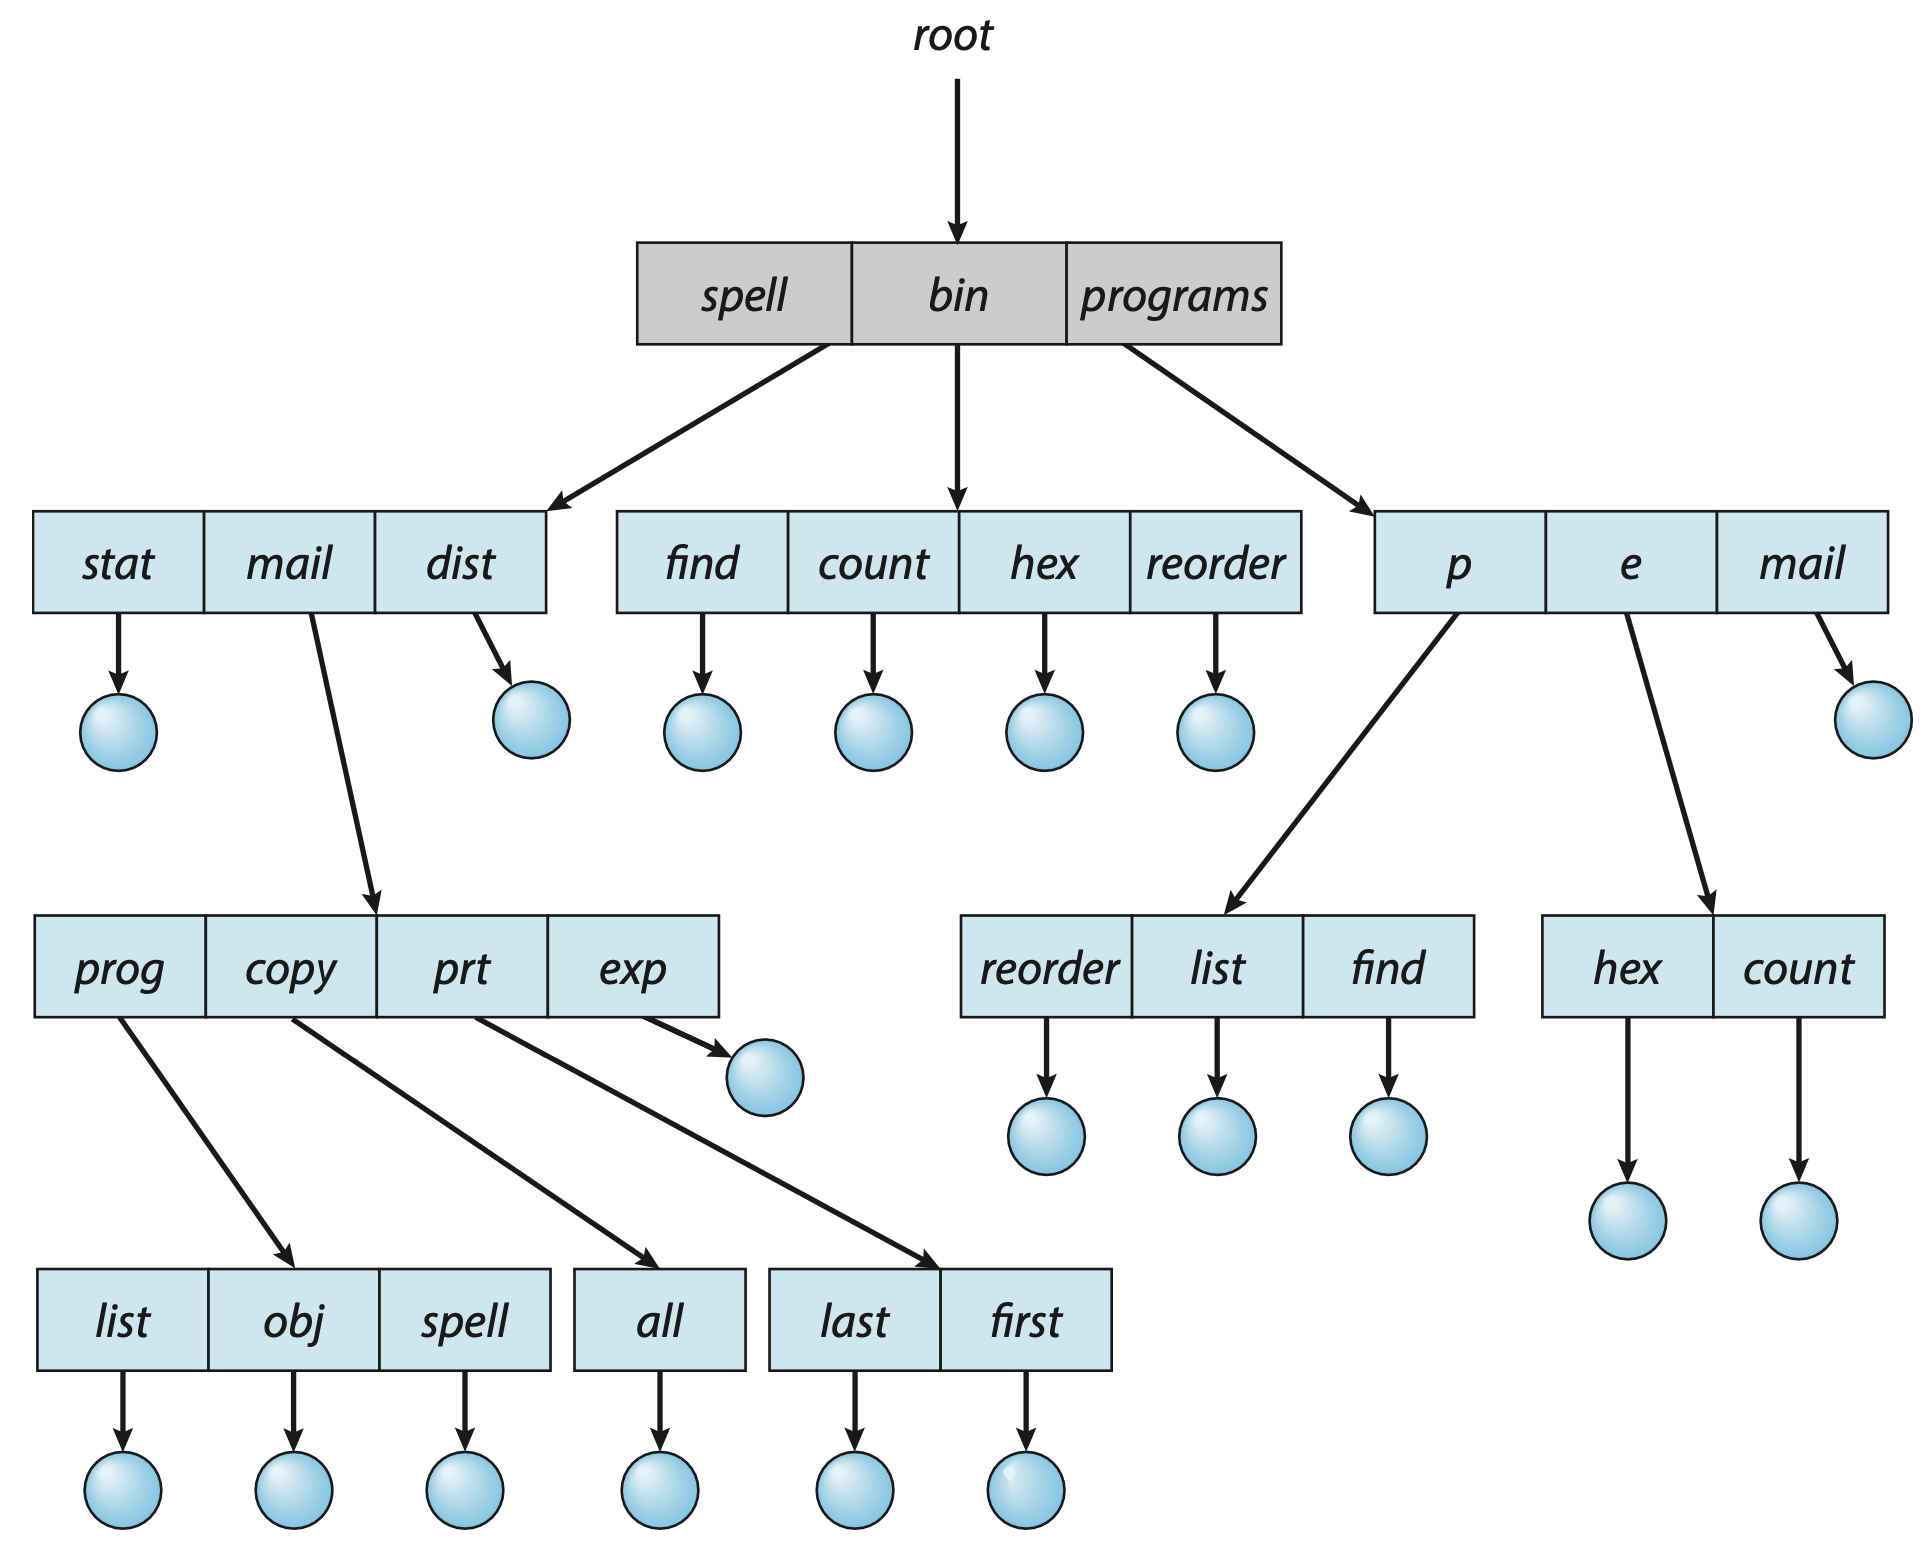
\includegraphics[width=0.6\linewidth]{figures/tree_dir.png}
                            \caption{Tree-Structured Directory}
                        \end{figure}
                    \subsubsection{Acyclic Graph Directory}
                        \begin{figure}[H]
                            \centering
                            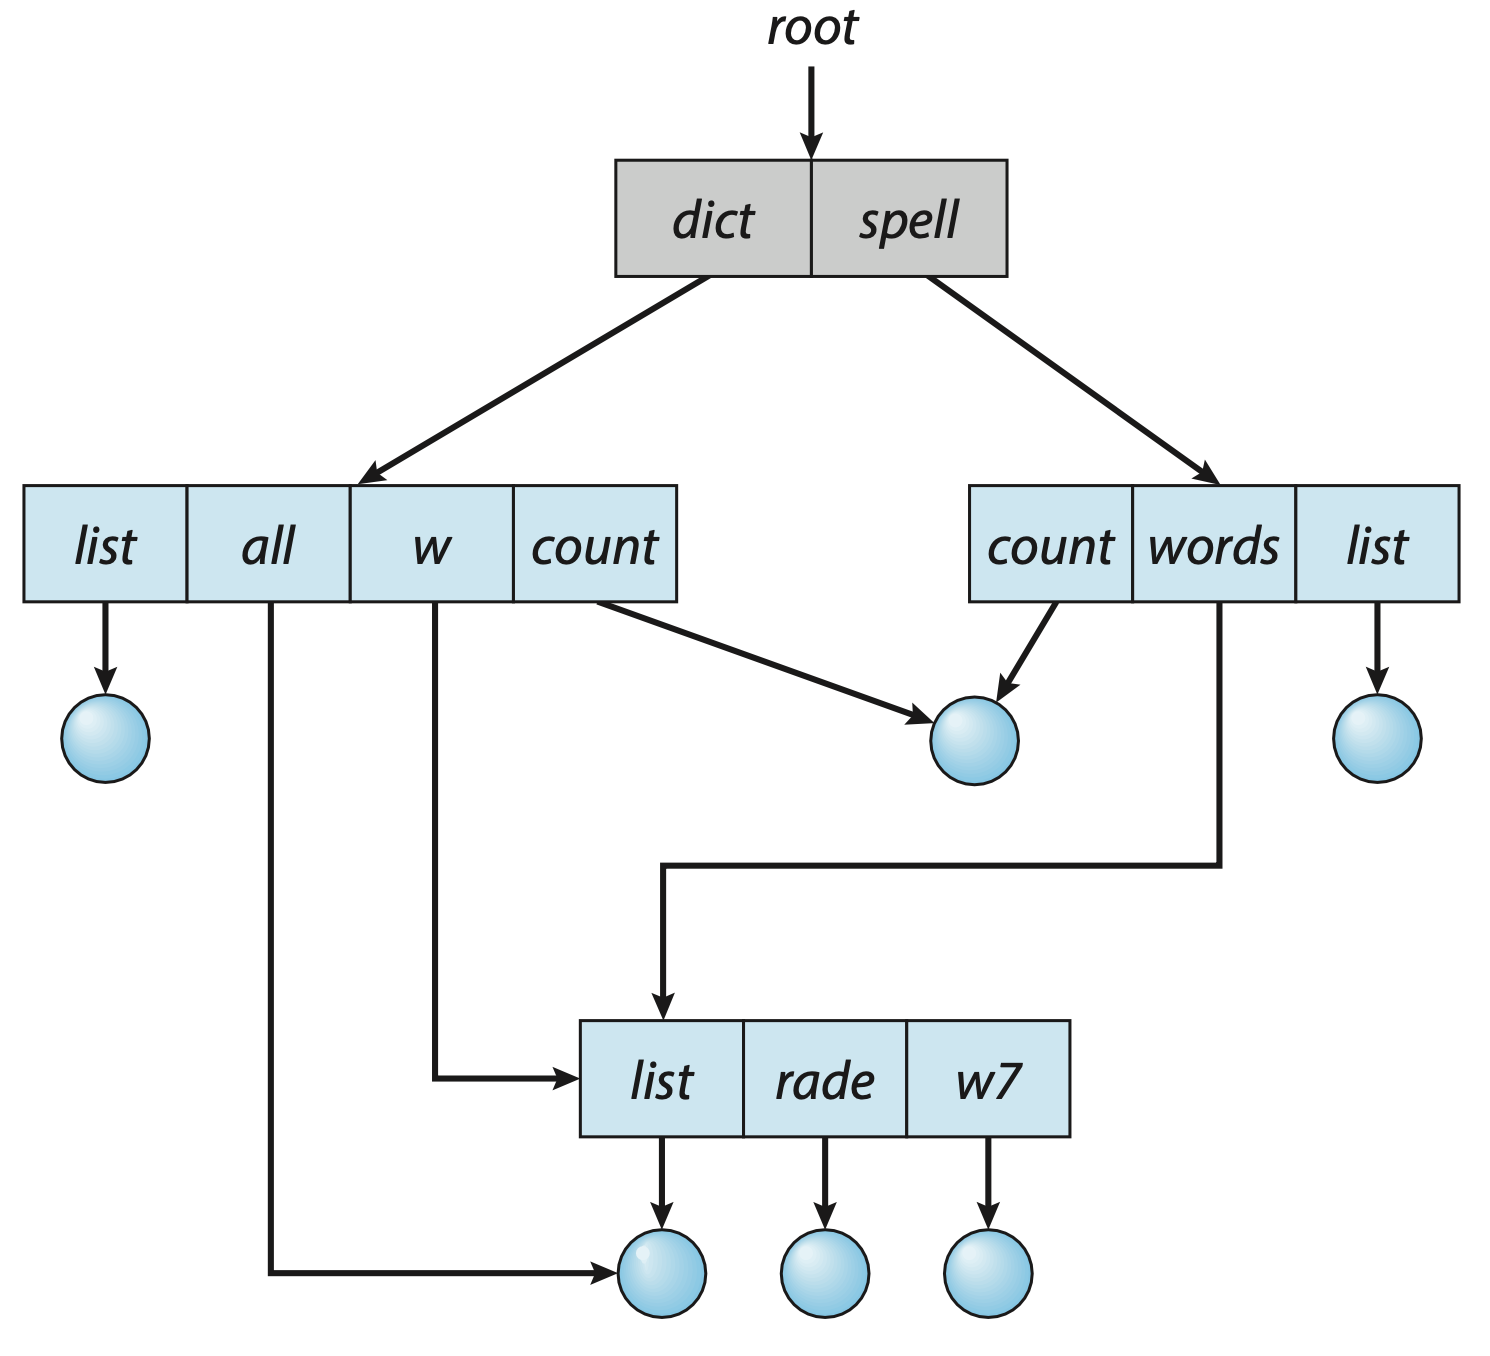
\includegraphics[width=0.6\linewidth]{figures/acyclic_graph_dir.png}
                            \caption{Acyclic Graph Directory}
                        \end{figure}
                    \subsubsection{General Graph Directory}
                        \begin{figure}[H]
                            \centering
                            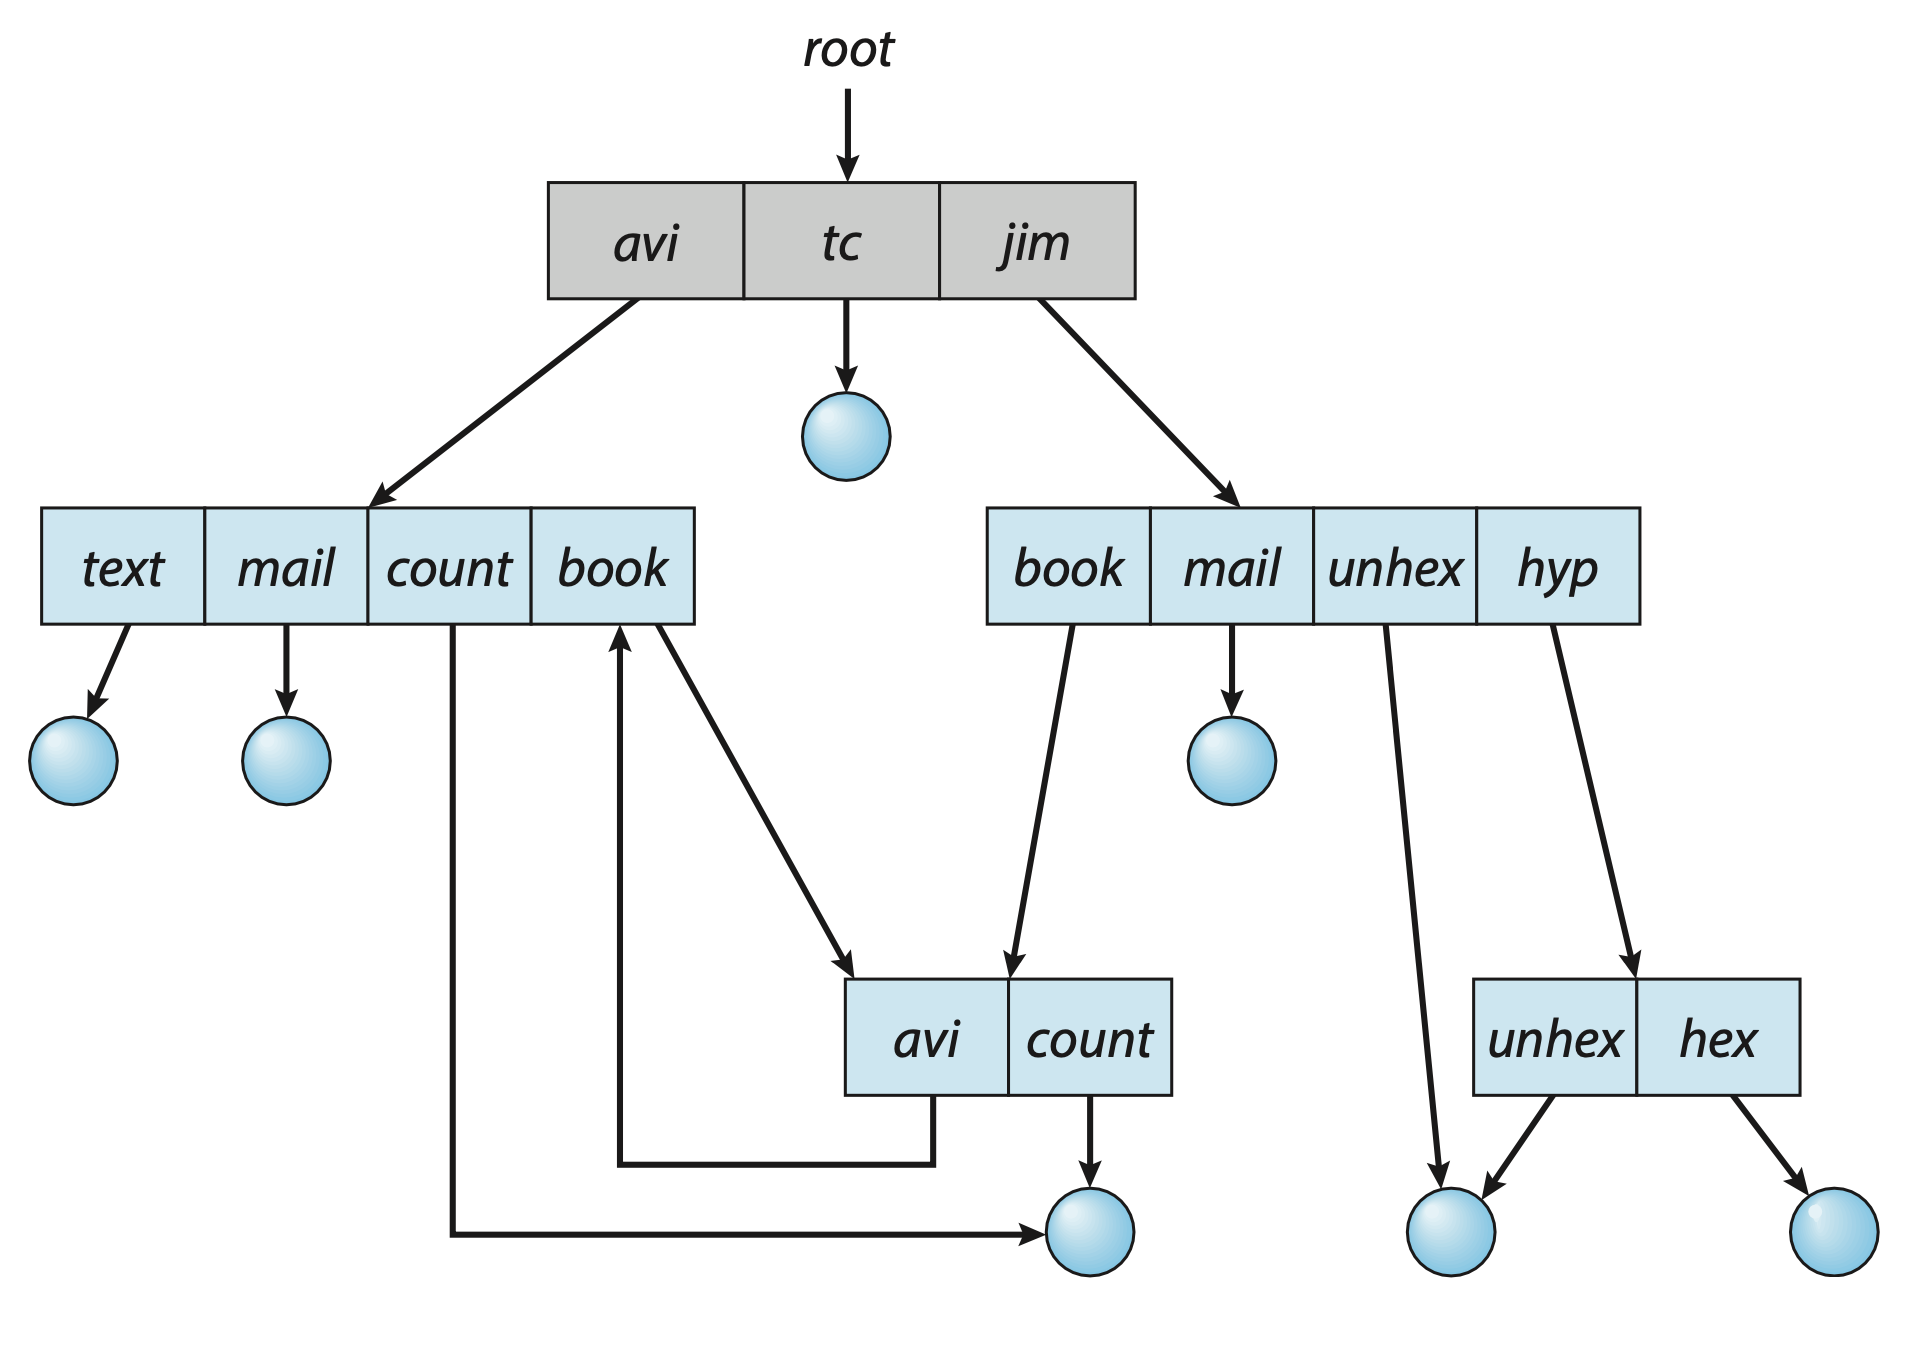
\includegraphics[width=0.6\linewidth]{figures/general_graph_dir.png}
                            \caption{General Graph Directory}
                        \end{figure}
                        
            % \subsection{File Sharing}
            \subsection{Protection}
                File owner/creator must be able to control what can be done and by whom.\\
                The following types of access have been defined for files
                \begin{itemize}
                    \item \textbf{Read}
                    \item \textbf{Write}
                    \item \textbf{Execute}
                    \item \textbf{Append}
                    \item \textbf{Delete}
                    \item \textbf{List}
                \end{itemize}
            \subsection{Access Lists and Groups}
                Modes of access: \textcolor{blue}{read, write, execute}.\\
                Three user classes in Unix
                \begin{figure}[H]
                    \centering
                    \begin{tabular}{ccc}
                        \textbf{User} & \textbf{Group ID} & \textbf{rwx} \\
                        \toprule
                        Owner & 7 & 111 \\
                        Group & 6 & 110 \\
                        Public & 1 & 001 \\
                    \end{tabular}
                    \caption{Unix Access Classes}
                \end{figure}
        % \section{File System Implementation}
        %     \subsection{File System Implementation}
        %     \subsection{Directory Implementation}
        %     \subsection{Allocation Methods}
        %     \subsection{Free-Space Management}
    \chapter{Virtual Machines}
        Virtual machines abstract the hardware of a single computer (CPU, memory, disk drives, network interface cards, etc.)
        into several execution environments, creating the illusion that each environment is running on its own computer.
        Virtualization creates a layer on which the operating system/applications can run.\\
        Virtual machine implmentations involve seperate components
        \begin{itemize}
            \item \textbf{Host} - the underlying hardware that runs the virtual machine
            \item \textbf{Virtual Machine Manager (VMM/Hypervisor)} - software that creates and runs 
            virtual machines by providing an interface identical to the host
            \item \textbf{Guest} - the operating system and/or applications running on the hypervisor
        \end{itemize}
        \section{Hypervisor}
            \subsection{Type 0 Hypervisor}
                Is an older idea with many names, including \textbf{bare metal}, \textbf{native}, \textbf{embedded}, \textbf{domains},
                and \textbf{partitions}.\\
                Hardware features are implemented by firmware. The hypervisor is the first software to run on the hardware and the operating
                system requires no modifications.\\
                Limited feature set but high performance as each guest gets dedicated hardware.\\
                I/O is difficult as the hypervisor must implement all drivers.\\
                VMM implements a \textcolor{blue}{control partition} that runs daeomsn that other guests communicate
                with for shared I/O.\\
                Allows for nesting virtualization, where a guest can run its own hypervisor and create its own guests.
            \subsection{Type 1 Hypervisor}
                Common in datacenters and cloud computing.\\
                Datacenter managers control and manage operating systems in new, sophisticated ways by controlling the Type 1
                hypervisor.\\
                Consolidation of multiple operating systems and apps onto less hardware.\\
                Move guests between systems to balance performance.\\
                Allows for snapshots and cloning.\\
                Rn in kernel mode, taking advantage of hardware protection. WHere the host CPU allows, they 
                use multiple modes to give the guest operating system individual control and improved performance.
                They are also operating systems of their own, and therefore have their own CPU scheduling,
                memory management, and I/O subsystems.\\
                Commonly closed source offerings (VMware ESX, Microsoft Hyper-V, Citrix XenServer)\\
                These can run on Type 0 hypervisors but not on other Type 1 hypervisors.\\
            \subsection{Type 2 Hypervisor}
                These are less interesting from an operating system's perspective as there is little involvement 
                in these.\\
                Run in the application level as VMMs and are simplyu another process that is run and managed by the host.\\
                The host is unaware that there is a VMM running.\\
                Have limits not associated with other types such as requiring superuser/administrator to access hardware assistance
                features of modern CPUs and cannot use these features if not given these permissions and have extra overhead
                of running.\\
                Have the benefit of being able to run on any host operating system and therefore can be used to test non native
                operating systems and software.
            \subsection{Paravirtualization}
            \subsection{Programming-Environment Virtualization}
            \subsection{Emulation}
            \subsection{Application Containment}
    \listoffigures
\end{document}
